%%%%%%%%%%%%%%%%%%%%%%%%%%%%%%%%%%%%%%%%%%%%%%%%%%%%%%%%%%%%
%%% LIVECOMS ARTICLE TEMPLATE FOR BEST PRACTICES GUIDE
%%% ADAPTED FROM ELIFE ARTICLE TEMPLATE (8/10/2017)
%%%%%%%%%%%%%%%%%%%%%%%%%%%%%%%%%%%%%%%%%%%%%%%%%%%%%%%%%%%%
%%% PREAMBLE
\documentclass[9pt,tutorial]{livecoms}
% Use the 'onehalfspacing' option for 1.5 line spacing
% Use the 'doublespacing' option for 2.0 line spacing
% Use the 'lineno' option for adding line numbers.
% Use the "ASAPversion' option following article acceptance to add the DOI and relevant dates to the document footer.
% Use the 'pubversion' option for adding the citation and publication information to the document footer, when the LiveCoMS issue is finalized.
% The 'bestpractices' option for indicates that this is a best practices guide.
% Omit the bestpractices option to remove the marking as a LiveCoMS paper.
% Please note that these options may affect formatting.

\usepackage{lipsum} % Required to insert dummy text
\usepackage[version=4]{mhchem}
\usepackage{siunitx,bm}
\usepackage{hyperref} % Not original - Added by Jack
\usepackage{listings} % Not original - Added by Jack
\DeclareSIUnit\Molar{M}
\usepackage[italic]{mathastext}
\newcommand{\pka}{p\textit{K}$_{\rm a}$}
\graphicspath{{figures/}}

%%%%%%%%%%%%%%%%%%%%%%%%%%%%%%%%%%%%%%%%%%%%%%%%%%%%%%%%%%%%
%%% IMPORTANT USER CONFIGURATION
%%%%%%%%%%%%%%%%%%%%%%%%%%%%%%%%%%%%%%%%%%%%%%%%%%%%%%%%%%%%

\newcommand{\versionnumber}{1.0}  
% you should update the minor version number in preprints and major version number of submissions.
\newcommand{\githubrepository}{\url{
https://github.com/JanaShenLab/CpHMD-Tutorial}}  %this should be the main github repository for this article

%%%%%%%%%%%%%%%%%%%%%%%%%%%%%%%%%%%%%%%%%%%%%%%%%%%%%%%%%%%%
%%% ARTICLE SETUP
%%%%%%%%%%%%%%%%%%%%%%%%%%%%%%%%%%%%%%%%%%%%%%%%%%%%%%%%%%%%
\title{A Guide to the Continuous Constant pH Molecular Dynamics 
Methods in Amber and CHARMM v[\versionnumber]}

\author[1,\authfn{1},\authfn{2}]{Jack A. Henderson}
\author[1,\authfn{1}]{Ruibin Liu}
% \alsoaffiliation{
% Joint first author
% }
\author[1,\authfn{3}]{Julie A. Harris}
\author[1,\authfn{4}]{Yandong Huang}
\author[1]{Vinicius Martins de Oliveira}
%\author[1]{Paween Mahinthichaichan}
\author[1*]{Jana Shen}
\affil[1]{University of Maryland School of Pharmacy, Baltimore, MD}
%\affil[2]{Institution 2}

\corr{jana.shen@rx.umaryland.edu}{JS}  % Correspondence emails.  FMS and FS are the appropriate authors initials.
%\corr{email2@example.com}{FS}

\orcid{Jack A. Henderson}{https://orcid.org/0000-0001-6675-7944}
\orcid{Ruibin Liu}{https://orcid.org/0000-0001-8395-9353}
\orcid{Julie A. Harris}{https://orcid.org/0000-0002-1130-6457}
\orcid{Yandong Huang}{https://orcid.org/0000-0002-1452-6383}
\orcid{Vinicius M. de Oliveira}{https://orcid.org/0000-0003-0927-3825}
\orcid{Jana Shen}{https://orcid.org/0000-0002-3234-0769}

\contrib[\authfn{1}]{These authors contributed equally to this work}
% \contrib[\authfn{2}]{These authors also contributed equally to this work}

\presentadd[\authfn{2}]{Scorpion Therapeutics, Boston, MA}
\presentadd[\authfn{3}]{ComputChem, Baltimore, MD}
\presentadd[\authfn{4}]{Jimei University, College of Computer Engineering, Xiamen, China}
% \presentadd[\authfn{4}]{Department, Institute, Country}

\blurb{This LiveCoMS document is maintained online on GitLab at \githubrepository. To provide feedback, suggestions, or help improve it, please visit the GitLab repository and participate via the issue tracker.}

%%%%%%%%%%%%%%%%%%%%%%%%%%%%%%%%%%%%%%%%%%%%%%%%%%%%%%%%%%%%
%%% PUBLICATION INFORMATION
%%% Fill out these parameters when available
%%% These are used when the "pubversion" option is invoked
%%%%%%%%%%%%%%%%%%%%%%%%%%%%%%%%%%%%%%%%%%%%%%%%%%%%%%%%%%%%
\pubDOI{10.XXXX/YYYYYYY}
\pubvolume{<volume>}
\pubissue{<issue>}
\pubyear{<year>}
\articlenum{<number>}
\datereceived{Day Month Year}
\dateaccepted{Day Month Year}

% \lstnewenvironment{listings}[1][] 
%  {\lstset{frame=off,escapechar=`,breaklines, breakindent=10pt, breakatwhitespace=True, linewidth=3.4in, #1}}
% {}

\lstnewenvironment{plaincontent}[1][] 
 {\lstset{frame=shadowbox,escapechar=`,breaklines, breakindent=10pt, breakatwhitespace=True, linewidth=3.4in, #1}}
{}
%%%%%%%%%%%%%%%%%%%%%%%%%%%%%%%%%%%%%%%%%%%%%%%%%%%%%%%%%%%%
%%% ARTICLE START
%%%%%%%%%%%%%%%%%%%%%%%%%%%%%%%%%%%%%%%%%%%%%%%%%%%%%%%%%%%%

\begin{document}

\begin{frontmatter}
\maketitle

\begin{abstract}
%This particular document provides a skeleton illustrating key sections for a Tutorial document.
%Please see the sample \texttt{sample-document.tex} in \url{github.com/livecomsjournal/article_templates/templates} for additional information on and examples of using the LiveCoMS LaTeX class.
%Here we also assume familiarity with LaTeX and knowledge of how to include figures, tables, etc.; if you want examples, see the sample just referenced.

%In your work, in this particular slot, please provide an abstract of no more than 250 words.
%Your abstract should explain the main contributions of your article, and should not contain any material that is not included in the main text.
%Please note that your abstract, plus the authorship material following it, must not extend beyond the title page or modifications to the LaTeX class will likely be needed.

% Begin Abstract Here
Like temperature and pressure, solution pH is an important environmental variable in biomolecular simulations. 
Virtually all proteins depend on pH to maintain their structure and function. 
In conventional molecular dynamics (MD) simulations of proteins, pH is implicitly accounted for by assigning and fixing protonation states of titratable sidechains. This is a significant drawback, 
as the assigned protonation states may be wrong and they may change during dynamics.
In this tutorial, we guide the reader in learning and using the various continuous constant pH MD methods in Amber and CHARMM packages, which have been applied to predict {\pka} values and elucidate proton-coupled conformational dynamics of a variety of proteins including enzymes and membrane transporters.
\end{abstract}

\end{frontmatter}


%Here you would explain what problem you are tackling and briefly motivate your work.


%Keep in mind, as you prepare your manuscript, that you should plan for a representative image  which will be used to highlight your article on the journal website and publications. Usually, this would be one of your figures, but it must also be uploaded separately upon article submission. We give specific guidelines for this image on the journal website in the section on article submission (see \url{https://livecomsjournal.github.io/authors/policies/index.html#article-submission}).

%Additionally, for well-formatted manuscripts, we recommend that you let LaTeX handle figure/table placement for you as much as possible, so please avoid specifying strenuous float instructions like `[h!]` and `[H]` as much as possible.





\section{Introduction} % - Vini 
\subsection{Background}
Solution pH is tightly regulated in biological environments \cite{Casey_Orlowski_2010_Nat.Rev.Mol.CellBiol.}. 
In normal adult cells, intracellular pH$_{\rm i}$ is about 7.2 and extracellular pH$_{\rm e}$ is about 7.4 \cite{Webb_Barber_2011_Nat.Rev.Cancer};
however, in cancer cells, the pH gradient is reversed,
which promotes cancer progression, metabolic adaptation, and metastasis
\cite{Webb_Barber_2011_Nat.Rev.Cancer,White_Barber_2017_J.CellSci.}. 
Virtually all proteins depend on pH to maintain their structure and function
\cite{Casey_Orlowski_2010_Nat.Rev.Mol.CellBiol.,Roos_Boron_1981_Physiol.Rev.}.
% Protein folding is one example of a pH-dependent process, where the unfolded protein only can reach its native state in a narrow pH range. 
A small change in pH can perturb the functions of many enzymes.
 %The protonation state of residues is also critical in drug design once the ligand-protein binding is susceptible to charge changes \cite{Dominguez_Sussman_2010_Biochemistry,Bax_Edge_2017_ActaCrystallogrDStructBiol}. 
For example, SARS coronavirus main proteases have the maximal
cleavage activity in a narrow pH range around 7.0 \cite{Tan_Hilgenfeld_2005_J.Mol.Biol.}. 
Below the optimum pH, the active site collapses
due to the protonation state change of a histidine \cite{Tan_Hilgenfeld_2005_J.Mol.Biol.,Verma_Shen_2020_J.Am.Chem.Soc.}. 
The function of human $\beta$-secretase 1 peaks at pH 4.5,
\cite{Shimizu_Nukina_2008_Mol.CellBiol.}; at low or high pH
the protonation state of the catalytic dyad changes, 
which results in the closure of the ``flap'' that lies above
the active site and blockage of 
substrate entrance \cite{Ellis_Shen_2015_J.Am.Chem.Soc.}.
%  the rational design of inhibitors must consider how the ligand interactions can alter the protonation state of the titratable residues into the binding site. 
Solution pH is also an important parameter in the creation of dynamic, stimuli-responsive materials \cite{Li_Payne_2019_Biofabrication}. 
For example, pH triggers the formation of hydrogel films
from the biopolymer chitosan
\cite{Morrow_Shen_2015_J.Am.Chem.Soc.}; 
addition of surfactants allows the chitosan film to be reconfigured via a second pH signal to achieve different mechanical properties \cite{Tsai_Shen_2018_Chem.Mater.}.

In a conventional molecular dynamics (MD) simulation,
solution pH is implicitly taken into account by
fixing the protonation states of titratable sites according to the experimental {\pka} values of
model compounds (or peptides) or 
traditional {\pka} calculations based on a static structure. 
Traditional {\pka} methods include empirical
approaches, e.g.,
PropKa \cite{Olsson_Jensen_2011_J.Chem.TheoryComput.},
Rosetta \cite{Kilambi_Gray_2012_Biophys.J.},
Poisson-Boltzmann solvers
MCCE \cite{Song_Gunner_2009_J.Comput.Chem.},
APBS/PDB2PQR \cite{Unni_Baker_2011_J.Comput.Chem.}, 
DelPhiPKa \cite{Wang_Alexov_2016_Bioinformatics},  
H++ \cite{Anandakrishnan_Onufriev_2012_NucleicAcidsRes.},
and other variants \cite{WarwickerJim_WarwickerJim_2011_Proteins}.
These tools are fast; however, 
the predicted protonation states are often incorrect
for deeply buried sites
\cite{Alexov_Word_2011_Proteins},
enzyme active sites \cite{Huang_Shen_2018_J.Phys.Chem.Lett.},
transmembrane proteins \cite{Huang_Shen_2016_Nat.Commun.},
and cysteines or lysines in general \cite{Liu_Shen_2019_J.Am.Chem.Soc.,Harris_Shen_2020_J.Chem.TheoryComput.,Liu_Shen_2021_J.Med.Chem.a}.
% due to a significant {\pka} shift in the protein environment relative to the solution (model) value.
% 2) Even if the assignment is correct based on the initial experimental structure, a change in protonation (or tautomer) state may occur during dynamics.. 
Also, even assuming an accurate assignment of protonation states at the beginning of MD, the conformational changes sampled
by the simulation may modify the electrostatic environment around the titratable groups, changing their protonation states. 
To account for 
the direct coupling between conformational dynamics and protonation state changes and to offer more accurate \pka\ predictions, constant pH MD methods have been developed.

Over the past two decades, much progress has been made in the
development of constant pH MD methods.
% Regarding the system modeling, the C$\alpha$ structure-based model CpHMD is one of the highest CG level approaches; such model treats amino acid residues as beads centered in $\alpha$ carbon, and titratable residues charge is also placed in the center of the bead.  
% \cite{Contessoto_Leite_2016_J.Chem.TheoryComput.}. 
% The titratable Martini is another example of CpHMD-CG, but in turn, it can treat each residue for several beads that represent a group of two to five heavy atoms \cite{Grunewald_Marrink_2020_J.Chem.Phys.}. 
% Finally, the most sophisticated models can explicitly treat all atoms of the system, but even with several ways to model the simulated systems, the CpHMD methods are grouped into discrete and continuous categories. 
% \cite{Chen_Khandogin_2008_Curr.Opin.Struct.Biol.,Chen_Shen_2014_Mol.Simulat.}. 
In a discrete (also known as stochastic) constant pH MD (DpHMD), the MD trajectory is periodically
interrupted by the Metropolis Monte-Carlo (MC) sampling of 
protonation states \cite{Baptista_Soares_2002_J.Chem.Phys.,Mongan_McCammon_2004_J.Comput.Chem.,Swails_Roitberg_2014_J.Chem.TheoryComput.,Stern_Stern_2007_J.Chem.Phys.,Chen_Roux_2015_J.Chem.TheoryComput.}. 
Here, protonation and deprotonation of titratable groups is
sampled discretely, assuming one of the two states. 
In contrast, the continuous constant pH MD (CpHMD) 
\cite{Lee_Brooks_2004_Proteins,Khandogin_Brooks_2005_Biophys.J.,Khandogin_Brooks_2006_Biochemistry,Wallace_Shen_2011_J.Chem.TheoryComput.,Wallace_Shen_2012_J.Chem.Phys.,Huang_Shen_2016_J.Chem.TheoryComput.}
treats the protonation states of ionizable sites using an auxiliary set of continuous titration coordinates based on an extended Hamiltonian $\lambda$-dynamics approach \cite{Kong_Brooks_1996_J.Chem.Phys.}. 
This method allows the system to escape local energy minima by transiently accessing the partially protonated states, which are unphysical.
Although the latter is a major caveat, the CpHMD method offers significantly faster convergence and importantly it can be implemented for implicit-, hybrid-, and fully explicit-solvent simulations.
On the contrary, although progress is being made, 
e.g., via the approach of nonequilibrium MD \cite{Stern_Stern_2007_J.Chem.Phys.,Chen_Roux_2015_J.Chem.TheoryComput.,Radak_Roux_2017_J.Chem.TheoryComput.}, 
it is very challenging to extend the Monte-Carlo based DpHMD method to fully explicit-solvent simulations
due to the low acceptance rate as a result of the 
large energy change.
%In this tutorial, we will focus on the CpHMD methods.

In the implicit-solvent constant pH scheme, sampling of both conformational dynamics and protonation states is performed in implicit solvent, typically a generalized-Born (GB) model.
Implementations of this scheme include the GBMV-
\cite{Lee_Brooks_2003_J.Comput.Chem.} and 
GBSW- \cite{Im_Brooks_2003_J.Comput.Chem.} based CpHMD \cite{Lee_Brooks_2004_Proteins,Khandogin_Brooks_2005_Biophys.J.,Khandogin_Brooks_2006_Biochemistry} in CHARMM  \cite{Brooks_Karplus_2009_J.Comput.Chem.},
and the GBNeck2-based CpHMD
\cite{Huang_Shen_2018_J.Chem.Inf.Model.,Harris_Shen_2019_J.Chem.Inf.Model.},
and the OBC-GB \cite{Onufriev_Bashford_2002_J.Comput.Chem.}
based DpHMD method 
\cite{Mongan_McCammon_2004_J.Comput.Chem.}
in Amber \cite{Case_Kollman_2018_}.
In the hybrid-solvent constant pH scheme, conformational sampling
is conducted with explicit solvent, while a continuum
electrostatic model, e.g., GB or Poisson-Boltzmann (PB)
is used to calculate the solvation forces 
on the $\lambda$ particles for the CpHMD methods
or the energy changes due to protonation-state change
for the DpHMD methods.
Implementations of this scheme include
the PB/TIP3P based stochastic DpHMD method
\cite{Baptista_Soares_2002_J.Chem.Phys.}
for GROMACS \cite{Spoel_Berendsen_2005_J.Comput.Chem.},
the GBSW/TIP3P based CpHMD method \cite{Wallace_Shen_2011_J.Chem.TheoryComput.}
in CHARMM \cite{Brooks_Karplus_2009_J.Comput.Chem.},
and the OBC-GB/TIP3P based DpHMD method 
\cite{Swails_Roitberg_2014_J.Chem.TheoryComput.}
in Amber \cite{Case_Kollman_2018_}.
Note, the GBSW/TIP3P based CpHMD method \cite{Wallace_Shen_2011_J.Chem.TheoryComput.} was extended to the treatment of transmembrane systems \cite{Huang_Shen_2016_Nat.Commun.} by incorporating the membrane GBSW model \cite{Im_Brooks_2003_Biophys.J.}.
Finally, an all-atom or fully explicit-solvent
CpHMD method was implemented in CHARMM
\cite{Brooks_Karplus_2009_J.Comput.Chem.}
as a part of the $\lambda$-dynamics functionality
in the BLOCK module (CPHMD$^{\rm MS\lambda D}$) 
by the Brooks group \cite{Goh_Brooks_2014_Proteins}
and as an extension to the GBSW and hybrid-solvent CpHMD 
methods in the PHMD module by the Shen group
\cite{Wallace_Shen_2012_J.Chem.Phys.,Huang_Shen_2016_J.Chem.TheoryComput.}.
The all-atom CpHMD method by the Shen group is the only one that includes titratable water to compensate for the net charge fluctuation as a result of proton titration in the CpHMD simulation
\cite{Chen_Shen_2013_Biophys.J.}.
An all-atom CpHMD implementation was also developed by the
Grubm\"{u}ller group
\cite{Donnini_Grubmuller_2016_J.Chem.TheoryComput.}
in GROMACS
\cite{Spoel_Berendsen_2005_J.Comput.Chem.}, although it has not been validated for a large number of proteins yet.
Currently, the only all-atom discrete constant pH method is based on nonequilibrium MD,
and it is implemented in NAMD \cite{Phillips_Schulten_2005_J.Comput.Chem.}
by the Roux group
\cite{Chen_Roux_2015_J.Chem.TheoryComput.,Radak_Roux_2017_J.Chem.TheoryComput.}.
% Below we will focus on the CpHMD implementations
% developed by the Shen group.

While accurate prediction of protonation states or {\pka} values is a goal, a major application of constant pH MD is to elucidate the mechanisms of pH-dependent or proton-coupled conformational dynamics. 
One can argue that the latter can also be studied by conventional fixed-protonation-state MD by running simulations with different protonation states.
While this may well be true when the switch of one protonation state is involved, the problem quickly becomes intractable 
when multiple titration sites are involved.
Furthermore,
the identity of the titratable site responsible for proton-coupled conformational changes is
often unclear, which makes the fixed-protonation-state approach unfeasible.
% For example,
% in the spider silk protein \cite{Wallace_Shen_2012_J.Phys.Chem.Lett.},
% the sodium-proton antiporter NhaA \cite{Huang_Shen_2016_Nat.Commun.,Henderson_Shen_2020_Proc.Natl.Acad.Sci.USA} and the proton-coupled drug efflux pump AcrB \cite{Yue_Shen_2017_J.Chem.TheoryComput.}.
Importantly, by running fixed-protonation-state MD one cannot obtain the {\pka} value for the conformational transition \cite{Wallace_Shen_2012_J.Phys.Chem.Lett.,Huang_Shen_2016_Nat.Commun.,Yue_Shen_2017_J.Chem.TheoryComput.,Henderson_Shen_2020_Proc.Natl.Acad.Sci.USA}, 
which can be compared with experiment to validate the microscopic details revealed by simulation.
% Constant pH methods have been reviewed in the past \cite{Chen_Khandogin_2008_Curr.Opin.Struct.Biol.,Wallace_Shen_2009_MethodsEnzymol.,Chen_Shen_2014_Mol.Simulat.}. In this tutorial 
% pH-dependent processes often involve the
% protonation state switches of multiple titratable sites, some of which may sample both protonated and deprotonated states.
% Examples include
% protein folding \cite{Khandogin_Brooks_2006_Proc.Natl.Acad.Sci.USA,Khandogin_Brooks_2007_Proc.Natl.Acad.Sci.USA}
% and pH-triggered self assembly of materials \cite{Morrow_Shen_2015_J.Am.Chem.Soc.}.

Table~\ref{Table:applications} summarizes the applications of the implicit-, hybrid-, and fully explicit-solvent CpHMD methods developed in the Shen group.
% Over the past decade, CpHMD simulations have been applied 
% to proteins in different environments \cite{Chen_Shen_2014_Mol.Simulat.,Radak_Roux_2017_J.Chem.TheoryComput.}. 
The implicit-solvent GBSW- and GBNeck2-CpHMD methods have been mainly applied to {\pka} predictions of proteins
\cite{Khandogin_Brooks_2006_Biochemistry,Wallace_Shen_2009_MethodsEnzymol.,Wallace_Shen_2011_Proteins,Harris_Shen_2019_J.Chem.Inf.Model.,Harris_Shen_2020_J.Chem.TheoryComput.},
while the hybrid-solvent and all-atom CpHMD methods have been additionally applied to elucidate the mechanisms of pH-dependent or proton-coupled conformational processes, e.g.,
protein unfolding
\cite{Yue_Shen_2018_Phys.Chem.Chem.Phys.},
structure-function relationships of proteases and kinases \cite{Ellis_Shen_2015_J.Am.Chem.Soc.,Tsai_Shen_2019_J.Am.Chem.Soc.,Ma_Shen_2021_J.Chem.Inf.Model.,Verma_Shen_2020_J.Am.Chem.Soc.,Henderson_Shen_2020_J.Chem.Phys.}, protein/ligand binding \cite{Ellis_Shen_2016_J.Phys.Chem.Lett.,Harris_Shen_2017_J.Phys.Chem.Lett.,Henderson_Shen_2018_J.Phys.Chem.Lett.}, 
conformational activation of transmembrane channels and transporters \cite{Chen_Shen_2016_J.Phys.Chem.Lett.,Yue_Shen_2017_J.Chem.TheoryComput.,Huang_Shen_2016_Nat.Commun.},
and materials \cite{Morrow_Shen_2015_J.Am.Chem.Soc.,Tsai_Shen_2018_Chem.Mater.}.
A recent application of GBNeck2-CpHMD method is the prediction of nucleophilic cysteine and lysine sites for targeted covalent drug design \cite{Liu_Shen_2019_J.Am.Chem.Soc.,Verma_Shen_2020_J.Am.Chem.Soc.,Henderson_Shen_2020_J.Chem.Phys.,Liu_Shen_2021_J.Med.Chem.a,Liu_Shen_2021_RSCMed.Chem.}. 
In this tutorial, we will discuss GBNeck2-CpHMD in Amber \cite{Huang_Shen_2018_J.Phys.Chem.Lett.,Harris_Shen_2019_J.Chem.Inf.Model.},
hybrid-solvent  \cite{Wallace_Shen_2011_J.Chem.TheoryComput.},
and particle-mesh Ewald (PME) all-atom CpHMD 
\cite{Huang_Shen_2016_J.Chem.TheoryComput.}
in CHARMM \cite{Brooks_Karplus_2009_J.Comput.Chem.}. 
% The GB-based CpHMD methods
% have been validated for a large number of proteins and the latter has additionally revealed the pH-dependent or proton-coupled mechanisms of various soluble and transmembrane proteins.

\begin{table*}
\begin{center}
\begin{tabular}{p{1.2in}p{3in}ll}
System &  Topic  & Method & Reference\\ 
\hline
\multicolumn{2}{l}{\bf Soluble proteins} & \\
Benchmark proteins &  {\pka} calculations & GBSW 
& \cite{Khandogin_Brooks_2006_Biochemistry,Wallace_Shen_2009_MethodsEnzymol.}\\
SNase  & Blind {\pka} predictions for 87 engineered mutant proteins   & GBSW & \cite{Wallace_Shen_2011_Proteins}\\
Peptides and mini-proteins & pH-dependent folding mechanisms & GBSW & \cite{Khandogin_Brooks_2006_Proc.Natl.Acad.Sci.USA,Khandogin_Brooks_2007_Proc.Natl.Acad.Sci.USA,Khandogin_Brooks_2007_J.Am.Chem.Soc.}\\
Benchmark proteins & {\pka} calculations & Hybrid & \cite{Wallace_Shen_2011_J.Chem.TheoryComput.}\\
NTL9, BBL & Unfolded states and unfolding mechanism & Hybrid& \cite{Shen_Shen_2010_J.Am.Chem.Soc.,Yue_Shen_2018_Phys.Chem.Chem.Phys.}\\
SNase   & {\pka} calculation for a deeply buried lysine; proton-coupled opening of the site   & Hybrid & \cite{Shi_Shen_2012_Biophys.J.}\\
Spider silk protein & pH sensing residues for dimerization & Hybrid & \cite{Wallace_Shen_2012_J.Phys.Chem.Lett.}\\
BACE1, BACE2, cathepsin D, renin, plasmepsin D & Acid/base roles of the catalytic dyad; binding-induced protonation state change of the inhibitor; pH-dependent conformational dynamics;
proton-coupled dynamics of binding site water;
pH-dependent 
inhibitor binding free energy calculations & Hybrid & \cite{Ellis_Shen_2015_J.Am.Chem.Soc.,Ellis_Shen_2016_J.Phys.Chem.Lett.,Ellis_Shen_2017_J.Comput.Chem.,Harris_Shen_2017_J.Phys.Chem.Lett.,Henderson_Shen_2018_J.Phys.Chem.Lett.,Ma_Shen_2021_J.Chem.Inf.Model.,Henderson_Shen_2021_J.Chem.Inf.Model.}\\
c-Src Kinase & Proton-coupled conformational change of the DFG motif & Hybrid & \cite{Tsai_Shen_2019_J.Am.Chem.Soc.}\\
% BACE1, cathepsin D &  pH-dependent binding free energy calculations & Hybrid & \cite{Harris_Shen_2017_J.Phys.Chem.Lett.}\\
Benchmark proteins & {\pka} calculations for Asp/Glu/His &  All-atom & \cite{Huang_Shen_2016_J.Chem.TheoryComput.} \\
% Plasmepsin & Dissect the pH-dependent interaction of the ligand binding site, identify proton coupled allostery, elucidate the catalytic roles of the active site & Hybrid-Solvent \\
Various enzymes & Prediction of proton donor and nucleophile and physical determinants & Hybrid & \cite{Huang_Shen_2018_J.Phys.Chem.Lett.}\\
Benchmark proteins & {\pka} calculations for Asp/Glu/His/Cys &  GBNeck2 & \cite{Huang_Shen_2018_J.Chem.Inf.Model.,Harris_Shen_2019_J.Chem.Inf.Model.}\\
Various kinases &  Prediction and rationalization of reactive Lys and Cys  & GBNeck2 & \cite{Liu_Shen_2019_J.Am.Chem.Soc.,Liu_Shen_2021_J.Med.Chem.,Liu_Shen_2021_RSCMed.Chem.}\\
Coronavirus papain-like proteases  &   Protonation states of His/Cys; proton-coupled conformational dynamics  & GBNeck2 & \cite{Henderson_Shen_2020_J.Chem.Phys.}\\
Coronavirus main proteases  & Protonation states of His and Cys; proton-coupled conformational change of the binding site & GBNeck2 & \cite{Verma_Shen_2020_J.Am.Chem.Soc.}\\
\multicolumn{2}{l}{\bf Transmembrane proteins} & \\
Proton channel M2 & Proton-coupled channel opening/closing & Membrane-hybrid & \cite{Chen_Shen_2016_J.Phys.Chem.Lett.} \\
Sodium/proton antiporter NhaA   & Identification of proton binding residues; proton-coupled conformational changes & Membrane-hybrid & \cite{Huang_Shen_2016_Nat.Commun.,Henderson_Shen_2020_Proc.Natl.Acad.Sci.USA} \\ Efflux pump AcrB  &  Identification of proton binding residues; proton-coupled conformational transitions & Membrane-hybrid & \cite{Yue_Shen_2017_J.Chem.TheoryComput.}  \\
$\mu$-opioid receptor & {\pka} calculation & Membrane-hybrid & \cite{Vo_Ellis_2021_Nat.Commun.,Mahinthichaichan_Shen_2021_JACSAu}\\
\multicolumn{2}{l}{\bf Materials} & \\
Various surfactants & {\pka} calculation in micelle & GBSW and hybrid& \cite{Morrow_Shen_2011_J.Phys.Chem.B} \\
Fatty acid & {\pka} calculation in micelle and bilayer & All-atom& \cite{Morrow_Shen_2014_J.Chem.Phys.} \\
Fatty acid & pH-dependent micelle/bilayer formation & Hybrid& \cite{Morrow_Shen_2012_J.Chem.Phys.,Morrow_Shen_2013_Langmuir}\\
Peptide & pH-dependent unfolding of $\beta$-sheets; phase transition {\pka} & All-atom &  \cite{Cote_Shen_2014_J.Phys.Chem.C}\\
Polysaccharide chitosan & Glucosamine titration; pH-dependent dissociation of a model crystallite; phase transition {\pka}; pH-dependent interaction with a surfactant & All-atom & \cite{Morrow_Shen_2015_J.Am.Chem.Soc.,Tsai_Shen_2018_Chem.Mater.}\\
\end{tabular}
\end{center}
\caption{\textbf{Applications of the continuous constant pH MD (CpHMD) methods.}
GBSW-CpHMD \cite{Khandogin_Brooks_2005_Biophys.J.,Khandogin_Brooks_2006_Biochemistry},
hybrid-solvent \cite{Wallace_Shen_2011_J.Chem.TheoryComput.} and membrane-enabled hybrid-solvent \cite{Huang_Shen_2016_Nat.Commun.} CpHMD methods are implemented in CHARMM \cite{Brooks_Karplus_2009_J.Comput.Chem.}.
The GRF \cite{Wallace_Shen_2012_J.Chem.Phys.,Chen_Shen_2013_Biophys.J.}
and PME \cite{Huang_Shen_2016_J.Chem.TheoryComput.}  based all-atom 
CpHMD methods are also implemented in CHARMM \cite{Brooks_Karplus_2009_J.Comput.Chem.} and they can be used with co-titrating ions \cite{Wallace_Shen_2012_J.Chem.Phys.} or water \cite{Chen_Shen_2013_Biophys.J.}.
GBNeck2-CpHMD \cite{Huang_Shen_2018_J.Chem.Inf.Model.,Harris_Shen_2019_J.Chem.Inf.Model.} method is implemented in Amber18 \cite{Case_Kollman_2018_}.
The pH replica-exchange protocol \cite{Wallace_Shen_2011_J.Chem.TheoryComput.}
was used for all applications except for those with GBSW-CpHMD where the temperature replica-exchange protocol \cite{Khandogin_Brooks_2006_Biochemistry} was used.
All implementations except for GBNeck2-CpHMD are for CPU computing.
}
\label{Table:applications}
\end{table*}
\subsection{The continuous constant pH molecular dynamics framework}

In continuous CpHMD, each titratable residue is assigned a titration coordinate, $\lambda_i$ \cite{Lee_Brooks_2004_Proteins,Khandogin_Brooks_2005_Biophys.J.}. 
We attribute to this coordinate an implicit function of an underlying coordinate $\theta_i$ such that $\lambda_i$ is bound between 0 and 1:
\begin{equation}
    \lambda_i = \sin^2\theta_i,
\end{equation}
where 0 and 1 represent the protonated and deprotonated states, respectively. 
Since $\lambda$ continuously evolves between 0 and 1,
in simulation analysis we apply cutoffs to define
protonated ($\lambda^P < 0.2$) and deprotonated states ($\lambda^U > 0.8$). 
Having the titration coordinate in place, we use an extended Hamiltonian to allow the simultaneous propagation of spatial (real) and titration (virtual) coordinates:

\begin{equation}
\begin{split}
\label{eq:Hamiltonian}
\mathcal{H}(\{\bm{r}_a\},\{\theta_i\})=
&\frac{1}{2}\sum_am_a\dot{\bm{r}}_a^2+\frac{1}{2}\sum_im_i\dot{\theta}_i^2+U^{\rm int}(\{\bm{r}_a\})\\
&+U^{\rm hybr}(\{\bm{r}_a\},\{\theta_i\})+\sum_iU^{\ast}(\theta_i),
\end{split}
\end{equation}
where $\bm{r}_a$ refers to the (x,y,z) coordinates
of atom $a$, and $\theta_i$ refers to the titration coordinate of titratable residue $i$. 
The two first terms of Eq.~\ref{eq:Hamiltonian} give the kinetic energies of real atoms and virtual $\lambda$ particles. 
$U^{\rm int}$ represent the titration-independent bonded and non-bond energies. 
The fourth term, $U^{\rm hybr}$, describes the 
non-bond energies, which are dependent on both spatial and titration coordinates. 
For the particle-mesh Ewald (PME) all-atom CpHMD
\cite{Huang_Shen_2016_J.Chem.TheoryComput.}
$U^{\rm hybr}$ includes only Coulomb and van der Waals (vdW) energies, while for
the implicit- and hybrid-solvent CpHMD methods $U^{\rm hybr}$ also includes the generalized Born (GB) energy:
 
 \begin{equation}
\label{eq:Uhybr}
\begin{split}
U^{\rm hybr}(\{\bm{r}_a\},\{\theta_i\})=U^{\rm elec}(\{\bm{r}_a\},\{\theta_i\}) 
+ U^{\rm vdW}(\{\bm{r}_a\},\{\theta_i\})\\
+ U^{\rm GB}(\{\bm{r}_a\},\{\theta_i\})
\end{split}
\end{equation}

The dependence of the electrostatic energy on the titration coordinates arises from the requirement that
the partial atomic charges on the titrating residue
are linearly interpolated  
between the values in the deprotonated and protonated states with respect to $\lambda$:

% Thus, we can write the charge on atom $j$, $q_j$, on the titrating residue $i$ as
%
\begin{equation}
q_j(\lambda_i) = (1-\lambda_i) q_j^{\rm prot} +  \lambda_i q_j^{\rm unprot},
\label{eq:qlamb}
\end{equation}
where $q_j$ refers to the partial charge of an atom $j$ in the titrating residue $i$.
As to vdW energies, the 
interactions involving a titratable proton are linearly attenuated with respect to $\lambda$:
\begin{equation}
U^{\rm vdW}_{ij}(\bm r_i, \bm r_j, \lambda_i) = (1-\lambda_i)U^{\rm vdW\ast}_{ij}(\bm r_i, \bm r_j),
\end{equation}
where $i$ is the index for the titratable proton, $j$ is the index for all other atoms, and $U^{\rm vdW \ast}_{ij}$ refers to the protonation independent vdW interaction energy. If both $i$ and $j$ are titratable protons,
the interaction is linearly attenuated by the $\lambda$ values of both:
\begin{equation}
U^{\rm vdW}_{ij}(\bm r_i, \bm r_j, \lambda_i, \lambda_j) = (1-\lambda_i)(1-\lambda_j)U^{\rm vdW\ast}_{ij}(\bm r_i, \bm r_j).
\end{equation}
Note, the vdW energy correction is small and typically neglected in constant pH methods except for the CpHMD methods implemented in CHARMM and Amber \cite{Khandogin_Brooks_2005_Biophys.J.,Wallace_Shen_2011_J.Chem.TheoryComput.,Huang_Shen_2016_J.Chem.TheoryComput.,Huang_Shen_2018_J.Chem.Inf.Model.,Harris_Shen_2019_J.Chem.Inf.Model.}.

Finally, the last term in Eq. \ref{eq:Hamiltonian} 
only affects titratable groups and is consisted of 
three biasing potentials:
\begin{equation}
\label{eq:biasingpotential}
U^{\ast}(\theta_i)=-U^{\rm mod}(\lambda_i)+U^{\rm barr}(\lambda_i)+U^{\rm pH}(\lambda_i).
\end{equation}

The first biasing potential $U^{\rm mod}$ describes a potential of mean force (PMF) of model titration along the $\lambda$-coordinate, where the model represents a fully solvent-exposed amino acid, i.e., a blocked single amino acid or a small peptide in solution.
According to the linear response theory, 
model PMF is (in GB solvent) or can be approximated (in explicit solvent) as a quadratic function:
\begin{equation}
\label{eq:Umod_1d}
U^{\rm mod}(\lambda_i)=A(\lambda_i-B)^2.
\end{equation}
Here $A$ and $B$ are parameters that can be determined through free energy calculation methods, such as thermodynamic integration (TI, see section Parameterization). 
By analogy, in the case of coupled double-site titration \cite{Khandogin_Brooks_2005_Biophys.J.}, e.g., histidine or carboxylic acid, the model PMF is second order in both $\lambda$ and $x$, where 
$x$ is a coordinate that represents the tautomer interconversion.
The two-dimensional PMF can be written as a bivariate polynomial,
%
\begin{equation}
\begin{split}
U^{\rm mod}(\lambda_i,x_i) =
&a_0 \lambda_i^2 x_i^2 + a_1 \lambda_i^2 x_i + a_2 \lambda_i x_i^2 + a_3 \lambda_i^2 \\
&+ a_4 x_i^2 + a_5 \lambda_i x_i + a_6 \lambda_i + a_7 x_i + a_8.
\end{split}
\label{eq:double}
\end{equation}
Here $x_{i}=\sin^{2}\theta^{x}_{i}$ is bound between 0 and 1, where $\theta^{x}_{i}$ is the underlying unbound
variable. 
%

$U^{\rm barr}$, the second biasing potential in Eq. \ref{eq:biasingpotential}, describes a barrier or penalty potential in the center of the titration coordinate, 
%
\begin{equation}
U^{\rm barr}(\lambda_i) = -4\beta\left(\lambda_i - \frac{1}{2} \right)^2,
\label{eq:Ubarr}
\end{equation}
where $\beta$ is a parameter that determines the height of the barrier. 
Adding the barrier potential serves to
increase the sampling time at the end-point states (e.g., $\lambda<0.2$ or $\lambda>0.8$) and therefore
minimizing the unphysical vdW and electrostatic interactions associated with mixed state 
(e.g., $0.2 \le \lambda \le 0.8$). 

$U^{\rm pH}$, the last term of Eq.~\ref{eq:biasingpotential} 
describes the pH dependence of the deprotonation free energy 
and is given by
%
\begin{equation}
U^{\rm pH}(\lambda_i)=ln(10)k_BT({\rm pH}-\textrm{p}{K_a}^{\rm mod})\lambda_i, 
\label{eq:UpH}
\end{equation}
% 
where $k_B$ is the Boltzmann constant, $T$ is the system temperature, and $\textrm{p}{K_a}^{\rm mod}$ is the model {\pka} for the titratable residue $i$.


\subsection{Scope} % - Ruibin 
This tutorial mainly covers two CpHMD methods that
have been extensively validated and applied to various real-life problems:
1) the hybrid-solvent CpHMD \cite{Wallace_Shen_2011_J.Chem.TheoryComput.}
in CHARMM \cite{Brooks_Karplus_2009_J.Comput.Chem.}
and
2) the GBNeck2 implicit-solvent CpHMD
\cite{Huang_Shen_2018_J.Chem.Inf.Model.,Harris_Shen_2019_J.Chem.Inf.Model.}
in Amber \cite{Case_Kollman_2018}. Currently, fully patched Amber 18 and 20 released versions are supported. GBNeck2-CpHMD patches to them can be downloaded from our \href{https://gitlab.com/shenlab-amber-cphmd/cphmd-patches}{cphmd-patches} repository. Details about how to apply them are described on that repository page.
The CHARMM hybrid-solvent CpHMD currently supports CPUs only, 
but the Amber GBNeck2-CpHMD supports both CPU or GPU computing.
We strongly recommend running the CpHMD simulations
via the pH replica-exchange protocol to significantly accelerate convergence of \pka's and conformational sampling; however, if desired, a single pH 
simulation or a set of independent pH simulations can also 
be conducted.

In addition to the above two methods, we will briefly
discuss the PME all-atom CpHMD method implemented in
CHARMM for CPU computing \cite{Huang_Shen_2016_J.Chem.TheoryComput.}
and in Amber for GPU computing (Harris, Liu, and Shen, unpublished data). 
We note, this tutorial does not cover the GBSW implicit-solvent CpHMD method in CHARMM 
\cite{Lee_Brooks_2004_Proteins,Khandogin_Brooks_2005_Biophys.J.,Khandogin_Brooks_2006_Biochemistry,Arthur_Brooks_2016_J.Comput.Chem.a}, which is available for both CPU and GPU computing.
The GBSW-CpHMD method with the temperature replica-exchange protocol has been extensively validated for protein \pka\ 
predictions and pH-dependent conformational dynamics.

\section{Prerequisites} % - Ruibin
CpHMD is a specialized MD technique, so the user should have some familiarity with MD simulations and especially with the Amber or CHARMM packages. 
Users with experience with other MD engines, such as Gromacs
\cite{Abraham_Lindahl_2015_SoftwareX}, NAMD\cite{Phillips_Tajkhorshid_2020_J.Chem.Phys.}, 
or OpenMM
\cite{Eastman_Pande_2017_PLoSComput.Biol.} 
are encouraged to go through the introductory tutorials for Amber or CHARMM to get started. 
Before running a CpHMD simulation, it is important to know your research objective. 
If the objective is to predict the {\pka} values of soluble proteins or their protonation states at a certain pH condition, GBNeck2-CpHMD 
\cite{Huang_Shen_2018_J.Chem.Inf.Model.,Harris_Shen_2019_J.Chem.Inf.Model.}
is the best choice and Amber \cite{Case_Kollman_2018}
experience is required. 
If the objective is to investigate the detailed proton-coupled conformational dynamics, ion transfer, protein-ligand binding/unbinding,
or transmembrane proteins, then 
the hybrid-solvent CpHMD  \cite{Wallace_Shen_2011_J.Chem.TheoryComput.,Huang_Shen_2016_Nat.Commun.} 
or the all-atom PME CpHMD \cite{Huang_Shen_2016_J.Chem.TheoryComput.}
in CHARMM
\cite{Brooks_Karplus_2009_J.Comput.Chem.}
should be used.
We note, a GPU-accelerated all-atom PME CpHMD 
implementation in Amber22 \cite{Case_Kollman_2022}
has been recently released \cite{Harris_Shen_Submitted}.
Like all computational chemistry calculations, it is important to know the system of interest
before attempting any simulations. 
With such knowledge, we can decide what salt concentration, temperature, pH range, and titratable residue types to use in CpHMD. Also, the research objective dictates the simulation length. For example, to predict protonation states, simulation can be run until the unprotonated fractions at all pH are converged, typically 10-50 ns per replica. If however, a large conformational transition is of interest, the simulation should be much longer. 

\subsection{Background knowledge}
Knowledge of classical MD is required to understand what we can and cannot achieve through a MD simulation. 
The user should also understand the parameters used in energy minimization, heating, equilibration, and production runs. 
Of course, chemistry knowledge of pH, {\pka}, and protonation states and how they may impact the physical properties of the specific biological or material system is essential for obtaining meaningful results.

CpHMD simulations are run on a workstation or high-performance computing (HPC) cluster under a Linux operating system. 
The user is expected to have a good knowledge of Linux commands for accessing and editing files, submitting jobs to servers, and retrieving simulation result files. 
Shell script and preferably also Python skills are required for pre- and post-processing files. 
For simulations on a HPC cluster, the user is required to be familiar with the specific batch scheduler and queuing system, e.g., SLURM (Simple Linux Universal Resource Manager), SGE (Sun Grid Engine), or PBS (Portable Batch System). 
The user is expected to know commands for submitting and checking the status of jobs.
The user is also expected to set environmental variables required for the specific MD engine.
Nowadays, a CpHMD job can also be performed on a workstation with a single or multiple GPUs. 
In this case, the user is required to use commands such as `nvidia-smi' to check the GPU status and `nvcc --version' to check the CUDA version as well. 
The user can use any data visualisation tool(s), but matplotlib in Python and Jupyter notebooks are recommended in our analysis tool set.  


\subsection{Software/system requirements} 
For GBNeck2-CpHMD, Amber16 is the minimum version. 
Requirements for installing Amber can be found in the \href{https://ambermd.org/Installation.php}{Amber website}. 
For the GPU version (pmemd.cuda), a Nvidia GPU card with at least compute compatibility sm3.0 should be installed with the latest driver. 
CUDA 10.1 is the primary CUDA version for running it but early versions from CUDA 7.5 also works. 
After successfully installing CUDA, it is important to set three environmental variables in Linux. 
\textbf{CUDA\_HOME} and \textbf{LD\_LIBRARY\_PATH} must point to the directories where the desired CUDA version is installed. 
We also need to specify \textbf{CUDA\_VISIBLE\_DEVICES} to GPU device indices. For example, 
\begin{lstlisting}
$ export CUDA_HOME=/usr/local/cuda-10.1
$ export LD_LIBRARY_PATH=
            /usr/local/cuda-10.1/lib64
$ export CUDA_VISIBLE_DEVICES=0,1
\end{lstlisting}
These variables will direct the Linux system to use the CUDA 10.1 version installed in the /usr/local directory.
In the example above two GPU cards are available,
and the indices 0 and 1 for CUDA\_VISIBLE\_DEVICES indicate the first and second GPU to use, respectively. 
Following installation of Amber, the user should set the environmental variable \textbf{AMBERHOME} to the Amber installation folder. 
\begin{lstlisting}
$ export AMBERHOME=/path_to_Amber_version_xx/
\end{lstlisting}

Before preparing CpHMD inputs of a protein system, 
we need to clean up and fix problems in the PDB file,
e.g., removing non-protein atoms, adding missing residues and atoms, and fixing non-canonical amino acid residues. 
To do that, we can use the Perl script convpdb.pl in \href{http://blue11.bch.msu.edu/mmtsb/Main_Page}{mmtsb tool set} \cite{Feig_Brooks_2004_J.Mol.Graph.Model.} or \href{https://github.com/openmm/pdbfixer}{pdbfixer} in OpenMM \cite{Eastman_Pande_2017_PLoSComput.Biol.}. 
For example, the following commands can be used 
to fix the file 1vii.pdb downloaded from RCSB (\href{www.rcsb.org}{www.rcsb.org}) \cite{Berman_Bourne_2000_NucleicAcidsRes.}.  
\begin{lstlisting}
$ convpdb.pl -nohetero -fixcoo -renumber 1 -out
amber -chain A -segname 1vii.pdb 
\end{lstlisting}
or 
\begin{lstlisting}
$ pdbfixer --add-atoms=heavy 
--keep-heterogens=none --add-residues
--replace-nonstandard 1vii.pdb
\end{lstlisting}
 Alternatively, we can use a homology modeling software such as \href{https://swissmodel.expasy.org/}{SWISS-MODEL} \cite{Waterhouse_Schwede_2018_NucleicAcidsRes.} to fix those problems especially when the number of continuously missing residues is large \cite{Waterhouse_Schwede_2018_NucleicAcidsRes.}.
 
 The next step is to add capping ligands ACE and NH2 to the N- and C-terminus and to modify ASP, GLU and HIS to AS2, GL2, and HIP residues if these residue types are set as titratable. For AS2 and GL2, a library file \href{https://gitlab.com/shenlab-amber-cphmd/cphmd-prep/-/blob/master/Files/phmd.lib}{phmd.lib} and a force field modification file \href{https://gitlab.com/shenlab-amber-cphmd/cphmd-prep/-/blob/master/Files/frcmod.phmd}{frcmod.phmd} are included in Ambertools after version 19 \cite{Case_Kollman_2018}, or we can load them to tLeap/Leap from the directory containing the two files. The last step is to use tLeap/Leap in Amber/ Ambertools to generate topology and parameter files. Our \href{https://gitlab.com/shenlab-amber-cphmd/cphmd-prep}{cphmd-prep} tool set uses the pdbfixer tool for the first step and can do all the aforementioned steps to prepare GBNeck2-CpHMD compatible input files. 

We use a Python-based \href{https://gitlab.com/shenlab-amber-cphmd/async_ph_replica_exchange}{asynchronous replica exchange} implementation for GPU pH replica-exchange simulations. 
Scripts in \href{https://gitlab.com/shenlab-amber-cphmd/cphmd-analysis}{cphmd-analysis} are used for analyzing CpHMD related files, including convergence checking, {\pka} calculation, and replica-exchange profiling. 
Some simple trajectory based analysis such as RMSD can also be done, but the users can use any tools, e.g., CPPTRAJ \cite{Roe_Thomas_2013_J.Chem.TheoryComput.}, PTRAJ \cite{Roe_Thomas_2013_J.Chem.TheoryComput.}, VMD \cite{Humphrey_Schulten_1996_J.Mol.Graph.}, and MDAnalysis \cite{Michaud-Agrawal_Beckstein_2011_J.Comput.Chem.}. 
% Note that these free tools usually depends on other free softwares, including OpenMM, Ambertools, scipy, pandas, matplotlib, etc. 
% The instructions on how to install those software are covered in their individual pages and not discussed here. 

A suggestion to use Python dependent packages is to use Anaconda or Miniconda. With them, the user can create a virtual environment specific for CpHMD related calculations. 
For example, after installing Anaconda or Miniconda, we can type 
\begin{lstlisting}[language=bash]
$ conda create --name cphmd python=3.7
\end{lstlisting}
Note that we choose Python version 3.7 because the OpenMM package currently only supports up to Python 3.7. 
Activate the environment named 'cphmd' by
\begin{lstlisting}[language=bash]
$ conda activate cphmd
\end{lstlisting}
Many packages can be installed through the conda and pip tool.
\begin{lstlisting}[language=bash]
$ conda install -c omnia pdbfixer parmed
$ conda install -c conda-forge ambertools
                 mdanalysis matplotlib 
$ conda install -c anaconda numpy scipy pandas 
$ pip install f90nml
\end{lstlisting}
Whenever the user wants to do some calculations or analysis related to CpHMD, they can activate this 'cphmd' virtual environment and use the installed tools without causing conflict with other software. 
% Python Packages and Version required for Async-Replica Exchange 
% Python Packages and Version required for the CpHMD-Analysis Lambda Parser

For running the hybrid-solvent CpHMD \cite{Wallace_Shen_2011_J.Chem.TheoryComput.}
in CHARMM \cite{Brooks_Karplus_2009_J.Comput.Chem.}
you will need to follow the installation instructions in the \href{https://www.charmm.org/archive/charmm/documentation/installation/}{CHARMM documentation}.
We suggest including the MPI and the Hamiltonian replica exchange options.
\begin{lstlisting}[language=bash]
 $ ./install.com gnu xxlarge M mpif90 +CMPI
 +REPDSTR +ASYNC_PME +GENCOMM
 \end{lstlisting}
If you want to install CHARMM on a local workstation for building and preparing systems or for running a single pH simulation, you can use the following installation command.
\begin{lstlisting}[language=bash]
 $ ./install.com gnu xxlarge
 \end{lstlisting}


% \section{Content and links}

% A tutorial will normally draw on additional files and materials; clearly indicate where and how these are available, with links, and how they are being archived for the long-term and maintained so they stay current.
% You will likely want to reference your GitHub repository as a central point to access all of this information, and then the GitHub repository may link out to other content as needed.

% \section{Checklists}
% Tutorials do not necessarily require the use of a checklist as in Best Practices documents; however, they can include these if desired.
% Several useful checklist formats are available, with examples presented in \texttt{sample-document.tex} in \url{github.com/livecomsjournal/article_templates/templates}.
% One example is shown here.

\section{Workflow for the hybrid-solvent CpHMD in CHARMM} 
As all MD simulations, CpHMD consists of three stages: system preparation, equilibration, and production.
We will explain each stage using a specific protein as an example. 
To follow along, the tutorial files for soluble proteins can be 
downloaded from our GitLab website \href{https://gitlab.com/shenlab-amber-cphmd/cphmd-tutorial/-/tree/main/hphmd_charmm}{cphmd-tutorial/hphmd\_charmm}
and for transmembrane proteins, 
the tutorial files can be downloaded from \href{https://gitlab.com/shenlab-amber-cphmd/cphmd-tutorial/-/tree/main/memb_hphmd_charmm}{cphmd-tutorial/memb\_hphmd\_charmm}.
We will use the pH replica-exchange protocol \cite{Wallace_Shen_2011_J.Chem.TheoryComput.}
in all the examples.

 %--------------------------------------------- 
\begin{figure*}[htb!]
    \centering
    \includegraphics[width=6.6in]{figs/workflow_scheme.pdf}
    \caption{\textbf{Overview of the CpHMD workflow} 
    %Step 5: Add 0 and 1 to the S range.
    %Titration plot, S ==> S_i
    }
    \label{fig:intro}
\end{figure*}
 %--------------------------------------------- 


%------------------------------------------------------------------------------------
\subsection{System Preparation}

To demonstrate CpHMD simulations of 
soluble proteins without retaining the crystal waters,
we use the mini-protein BBL as an example.
The tutorial files for system preparation can be found 
in the directory
\href{https://gitlab.com/shenlab-amber-cphmd/cphmd-tutorial/-/tree/main/hphmd_charmm/bbl_sys_prep}{bbl\_sys\_prep}.

\begin{checklist}{Input files for preparation of a soluble protein}
%\begin{checklist}{Files Produced}
%\textbf{A list of files needed for the equilibration of a soluble protein}
\begin{itemize}
% \item System coordinates (.pdb/.crd)
% \item System topology (.psf)
%%\item Crystal Image Transformations (crystal$\_$image.str)
% \item Periodic boundary conditions (.pbc)
\item step1\_add\_h.inp
\item step2a\_make\_waterbox.inp
\item step2b\_solvate.inp 
\end{itemize}
\end{checklist}

\paragraph{Step 1. Prepare a protein structure with dummy hydrogens.}
First, we retrieve the coordinates of a protein structure
from \href{https://www.rcsb.org/}{Protein Data Bank}\cite{Berman_Bourne_2000_NucleicAcidsRes.},
e.g., BBL (PDB: 1w4h \cite{Ferguson_Fersht_2005_J.Mol.Biol.}).
A homology modeling tool such as SWISS-MODEL\cite{Waterhouse_Schwede_2018_NucleicAcidsRes.} 
can be used to add any missing atomic coordinates.
Next, we convert the PDB file from the standard PDB format to the CHARMM PDB format using the MMTSB tool command \cite{Feig_Brooks_2004_J.Mol.Graph.Model.} \href{http://blue11.bch.msu.edu/mmtsb/convpdb.pl}{convpdb.pl}
or a user supplied script followed by a shell command ``sed'' to
change all histidine residue names to HSP to facilitate titration.

%
\begin{lstlisting}
$ perl convpdb.pl -out charmm22 -segnames
-renumber 1 1w4h.pdb | sed "s/HSD/HSP/g" 
> start.pdb
\end{lstlisting}
%
Here, the output PDB file is formatted for CHARMM (-out charmm22); the segment names are included in the output (-segnames); the residue identification numbers (resid) are renumbered starting at 1; and 
the input file is "1w4h.pdb."
The CHARMM default tautomer for His is HSD.
Changing HSD to HSP indicates to the CpHMD program that histidine is titratable (see later discussion of the parameter file).
Although all resid have been renumbered starting from 1, this does not have to be the case.
Next we add hydrogen atoms to the protein using the HBUILD facility\cite{Brunger_Karplus_1988_Proteins} in CHARMM
\cite{Brooks_Karplus_2009_J.Comput.Chem.}.

To allow titration of Asp and Glu sidechains, we place dummy hydrogens on both carboxylate oxygens.
Note, the dummy atoms do not interact with each other 
and only one is turned on when Asp/Glu is protonated
\cite{Khandogin_Brooks_2005_Biophys.J.}.
The dummy hydrogens are placed in the \textit{syn} position, 
because it is considered
more favorable than the \textit{anti} position
(see discussion in Ref \cite{Khandogin_Brooks_2005_Biophys.J.}).
To prevent the dummy hydrogens from moving to the \textit{anti} position, in which case nonnative hydrogen bonds may form
and a neutral dummy may lose the ability to gain charge,
in the CpHMD specific force field parameter file,
the C--O bond rotation energy barrier
is increased from the standard 0.5 to 6.0 kcal/mol
(see discussion in Ref \cite{Khandogin_Brooks_2005_Biophys.J.}).

Following the addition of hydrogens, a brief energy minimization is performed to correct unfavorable positions.
Here 50 steps of steepest descent (SD) and 10 steps of adopted basis Newton-Raphson (ABNR) are used, whereby a harmonic restraint with the force constant of 50 kcal/mol/{\AA}$^2$ is placed on the heavy atoms.
In most cases the N- and C-terminal ends of the protein are truncated and require capping. 
For N-terminus, we use CH$_3$CO (patch ACE) and 
for C-terminus we use NH$_2$ (patch CT2) or NHCH$_3$ (patch CT3).
In special cases, the free ionized form, NH$_{3}^{+}$ and COO$^+$, is used and can be set titratable when CpHMD is turned on. 
The input file `step1a\_add\_h\_prot.inp' is an example of how to perform these steps on BBL and can be run with the following command.
%
\begin{lstlisting}[language=bash]
$ charmm -i step1a_add_h_prot.inp -o step1a.out
\end{lstlisting}
%
The example input also checks for disulfide bonds using a sulfur-to-sulfur distance cutoff of 2.5 {\AA}. 
After running any input file, make sure to visualize the output 
structure to confirm all the dummy hydrogens and additional features are correctly constructed. 

\paragraph{Step 2. Prepare a solvated system}
Now we move to protein solvation by first building a large 
water box of the desired size.
This is done by generating a plane of small cubic water boxes 
along the x- and y-axes, and then stacking the planar water boxes along the z-axis.
CHARMM toppar directory contains the cubic water box made
of pre-equilibrated TIP3P waters.
The size of the large water box is calculated based on the longest
dimension of the protein and a padding space between the protein 
and the edges of the water box.
We recommend having at least $\sim$10{\AA} padding in x, y, and z directions.
The large cubic water box is then reshaped to a truncated octahedron by removing waters in all eight corners. 
The input file `step2a\_make\_waterbox.inp' is used to construct the octahedron water box.
%
\begin{lstlisting}[language=bash]
$ charmm -i step2_make_waterbox.inp -o 
step2_make_waterbox.out
\end{lstlisting}
%
Once the water box is built, the protein is placed at the center and water molecules within 2.8 {\AA} of the protein heavy atoms are deleted.

The solvated system is subject to energy minimization to release unfavorable contacts. 
First, the protein heavy atoms are fixed and the system undergoes energy minimization using SD and ABNR for 50 steps each. 
Next, a five-stage minimization is conducted with the harmonic constants
of 100, 50, 25, 5, and 0 kcal/mol on the protein heavy atoms using 50 steps of SD and 100 steps of ABNR in each stage. 
The input file
``step3\_solvate.inp'' 
can be used.
%
\begin{lstlisting}[language=bash]
$ charmm -i step2b_solvate.inp -o
step2b_solvate.out
\end{lstlisting}
%
Again, always remember to visualize the system and make sure the system has been constructed to your expectations. 

\subsection{System preparation that includes crystal waters}

\begin{checklist}{Required inputs}
%\begin{checklist}{Files Produced}
%\textbf{A list of files needed for the equilibration of a soluble protein}
\begin{itemize}
% \item System coordinates (.pdb/.crd)
% \item System topology (.psf)
%%\item Crystal Image Transformations (crystal$\_$image.str)
% \item Periodic boundary conditions (.pbc)
\item step1a\_add\_h\_prot.inp
\item step1b\_add\_h\_crys\_wat.inp
\item step1c\_merge\_prot\_crys\_wat.inp
\item step2a\_make\_waterbox\_crys\_wat.inp
\item step2b\_solvate\_crys\_wat.inp 
\end{itemize}
\end{checklist}

In some cases the X-ray structure contains water molecules and it is desirable to keep them, e.g., those in the enzyme active site.
A tutorial showing how to set up a system with crystal waters can be
found in the directory \href{https://gitlab.com/shenlab-amber-cphmd/cphmd-tutorial/-/tree/main/hphmd_charmm/crys_wat_system_prep}{crys\_wat\_system\_prep}.
Here we use a small protein, staphylococcus nuclease (SNase), as an example,
as the X-ray structure (PDBid: 3hzx) contains crystal waters.
% In the previous example, the solution NMR structure of BBL did not contain crystal waters.\cite{Ferguson_JMolBiol_2005_v353_p427}
To keep the crystal waters, just a few additional steps are needed.
First, move all the water molecules into a separate PDB file and make sure the file is properly formatted with the correct column names and column spacing.
In the tutorial the crystal water coordinates have been exported into the the file 'xwat$\_$original.pdb'; however, this file needs to be formatted for use in CHARMM. 
The Python script 'mod$\_$xwat.py' reformats this file, and in the example the reformatted file is named 'xwat$\_$final.pdb', and you might be able to modify the script for your simulation needs.
Most error messages involving the handling of crystal waters are due to the PDB file not being properly formatted. 

Since the crystal waters resolved in a X-ray structure do not contain hydrogen positions, they can be added using the CHARMM input file 'step1b$\_$add$\_$h$\_$xwat.inp'.
With hydrogens added to the protein and crystal waters, the two sets of coordinates need to be combined using the CHARMM input file 'step1c$\_$merge$\_$prot$\_$xwat.inp'.
The rest of the system preparation is very similar to
that without crystal waters.
The only difference to note is when you solvate the system you can merge the segids of the crystal waters (segid: XWAT) with the bulk water (segid: SOLV) using the following command.
%
\begin{lstlisting}[language=bash]
JOIN XWAT SOLV renumber
RENAME SEGID SOLV sele segid XWAT end
\end{lstlisting}
%
Keep in mind this needs to be done after the deletion of water that overlaps with the protein; otherwise you run the risk of accidentally removing some crystal waters.
An example of this is the input file 'step2b$\_$solvate$\_$crys$\_$wat.inp'.


\subsection{System preparation for transmembrane proteins}

\begin{checklist}{Required inputs}
 \begin{itemize}
 \item step1-5/*.inp
  \item step6/*.inp
% \item System Atom Coordinates (.pdb/.crd)
% \item System Atom Topology (.psf)
% \item System Assemtion nbly Info. (.str)
% \item Crystal Image Transformations (crystal$\_$image.str)
% \item Periodic Boundary Conditions (.pbc)
% \item Pre-Equil. System Coordinates (.crd/.pdb)
% \item Pre-Equil. System Trajectory (.dcd)
% \item Pre-Equil. System Information (.out)
% \item Pre-Equil. System Energies (.ene)
% \item Pre-Equil. System Restart (.rst)
\end{itemize}
\end{checklist}
Due to the presence of a lipid bilayer, the preparation of transmembrane proteins for CpHMD simulations requires additional steps.
We divide the preparation into the initial and final stages.
% First, we assemble the system including the protein
% and the solvated lipid bilayer followed by the relaxation of the bilayer. 
The related files can be accessed from the directories
\href{https://gitlab.com/shenlab-amber-cphmd/cphmd-tutorial/-/tree/main/memb_hphmd_charmm/initial_system_prep/}{initial\_system\_prep}
and \href{https://gitlab.com/shenlab-amber-cphmd/cphmd-tutorial/-/tree/main/memb_hphmd_charmm/final_system_prep/}{final\_system\_prep}.

In the initial system preparation, a solvated protein-membrane system is built.
%we first prepare the protein structure using `step1\_genpsf.inp'.
We start by retrieving the protein structure from the database \href{https://opm.phar.umich.edu/}{OPM} (Orientations of Proteins in Membranes), which properly orients the protein in the lipid bilayer using theoretical calculations and experimental data.\cite{Lomize_Mosberg_2006_Bioinformatics}
Just like for soluble proteins, any missing residues need to be added.
%and then the missing hydrogens can be added.
Here we adopt the standard protonation states, i.e., Asp(-), Glu(-), Cys(0), Lys(+), and Arg(+).
As the solution or model {\pka} of His is 6.54 \cite{Thurlkill_Pace_2006_ProteinSci.}, 
which is within one unit of the physiological pH, special attention needs to be given to its protonation (singly or doubly protonated) and tautomeric state (HSD or HSE), based on the nearby hydrogen bonding or salt-bridge interaction. 
% The protonation state of His can be set by changing the residue name in the PDB file and running the script. 
Like soluble proteins, the N- and C-terminal ends may be capped or if necessary the charged forms may be used. 

With the complete protein structure (all heavy atom positions
are in place), we use the script
\href{https://gitlab.com/shenlab-amber-cphmd/cphmd-tutorial/-/tree/main/memb_hphmd_charmm/initial_system_prep/step1-5}{step1\_genpsf.inp} to build
hydrogen positions followed by a short energy minimization in the GB implicit-solvent model to adjust any energetically
unfavorable hydrogen positions.
Next, we build the rest of the system and equilibrate the
lipid bilayer
following the CHARMM-GUI protocol for placing the lipids, solvating the system, and adding ions.\cite{Jo_Im_2007_PLoSONE}
The input files for these steps can be found in the directory \href{https://gitlab.com/shenlab-amber-cphmd/cphmd-tutorial/-/tree/main/memb_hphmd_charmm/initial_system_prep/step1-5}{step1-5}.
Below we will briefly go through the steps.

After the protein structure is prepared, we 
place it at the origin and estimate its 
cross section using the script
\href{https://gitlab.com/shenlab-amber-cphmd/cphmd-tutorial/-/tree/main/memb_hphmd_charmm/initial_system_prep/step1-5}{step2.1$\_$orient.inp}. 
The next step is to add water to the pore of the protein 
using the script \href{https://gitlab.com/shenlab-amber-cphmd/cphmd-tutorial/-/tree/main/memb_hphmd_charmm/initial_system_prep/step1-5}{step2.2$\_$pwat.inp}.
To determine the system dimensions the script \href{https://gitlab.com/shenlab-amber-cphmd/cphmd-tutorial/-/tree/main/memb_hphmd_charmm/initial_system_prep/step1-5}{step3.1$\_$size.inp} is used. This script also assesses the lipid type area and the number of lipids required to be placed between the protein boundary and the periodic boundary condition. 
Approximately 4 to 5 lipids should be placed between the protein and the PBC. 
Additionally, the script will state the thickness of the water slab above and below the lipid bilayer. 
With the dimensions of the system calculated, the lipid heads using big dummy spheres are placed to estimate the positions of the lipids in the bilayer. This is accomplished by \href{https://gitlab.com/shenlab-amber-cphmd/cphmd-tutorial/-/tree/main/memb_hphmd_charmm/initial_system_prep/step1-5}{step3.2$\_$packing.inp}.
Then the dummy spheres are replaced with lipid molecules from a library of randomized conformations using the script \href{https://gitlab.com/shenlab-amber-cphmd/cphmd-tutorial/-/tree/main/memb_hphmd_charmm/initial_system_prep/step1-5}{step4.1$\_$lipid.inp}.
In this example 1-palmitoyl-2-oleoyl-sn-glycero-3-phosphocholine (POPC) lipids are used, but if different lipids are needed other libraries of randomized conformations of lipid molecules can be found on the \href{https://www.charmm-gui.org/?doc=archive&lib=lipid}{CHARMM-GUI Archive - Individual Lipid Molecule Library}.

Next, a rectangular water box is generated using the input file \href{https://gitlab.com/shenlab-amber-cphmd/cphmd-tutorial/-/tree/main/memb_hphmd_charmm/initial_system_prep/step1-5}{step4.2$\_$waterbox.inp}, which solvates the protein and membrane complex.
Next the number of ions required to achieve the desired salt concentration is calculated and randomly placed in the slabs of water above and below the protein and membrane complex. 
In the final step, \href{https://gitlab.com/shenlab-amber-cphmd/cphmd-tutorial/-/tree/main/memb_hphmd_charmm/initial_system_prep/step1-5}{step5$\_$assembly.inp}, all of the system components are combined.
After the system is built, 
all components of the system are relaxed in six equilibration stages with gradually decreased harmonic restraint potentials using the scripts  \href{https://gitlab.com/shenlab-amber-cphmd/cphmd-tutorial/-/tree/main/memb_hphmd_charmm/initial_system_prep/step6}{step6.1$\_$equi.inp to 'step6.6$\_$equi.inp}.

Now we move to the final system preparation stage

%--------------------------------------------------------------------------------
\subsection{Equilibration of soluble proteins}
%--------------------------------------------------------------------------------

\begin{checklist}{Files Required}
%\textbf{A list of files needed for the equilibration of a soluble protein}
\begin{itemize}
% \item System Atom Coordinates (.crd)
% \item System Atom Topology (.psf)
% \item Periodic Boundary Conditions (.pbc)
\item equil\_hphmd.inp
%\item C22 Protein Topologies Parameters (.rtf/.prm)
%\item Water/Ion Topologies and Parameters (toppar$\_$water$\_$ions.str)
%\item C22 Hybrid PHMD Parameters (toppar$\_$phmd$\_$c22.str)
%\item Hybrid PHMD Parameters (phmd$\_$hybrid$\_$g2$\_$c22.in)
%\item GBSW Radii (radius$\_$gbsw.str)
\end{itemize}
\end{checklist}

% \begin{checklist}{Files Produced}
% %\textbf{A list of files needed for the equilibration of a soluble protein}
% \begin{itemize}
% \item Lambda Values (.lamb)
% \item Trajectory (.dcd)
% \item Energy Outputs (.ene)
% \item Restart (.rst)
% \end{itemize}
% \end{checklist}

Equilibration of soluble proteins for CpHMD is performed at a single pH in several stages. 
An example input for the BBL protein is
\href{https://gitlab.com/shenlab-amber-cphmd/cphmd-tutorial/-/tree/main/hphmd_charmm/bbl_equil_prod}{equil\_hphmd.inp}.
% , `\href{https://gitlab.com/shenlab-amber-cphmd/cphmd-tutorial/-/tree/main/hphmd_charmm/bbl_equil_prod}{equilibration$\_$hphmd.inp}.'
Since CpHMD is turned on during equilibration, titratable residues must be chosen. 
In the example here, Asp, Glu, and His are allowed to titrate because of the pH range used in the production simulation.
The crystal structure pH condition or physiological pH 7.4 can be used.
We specify the physiological ionic strength of 0.15 M and temperature of 298 K.
Before invoking the PHMD module for CpHMD
simulation, we need to call GBSW using the following command.
%
\begin{lstlisting}
GBSW HYBRID SGAMMA 0.005 NANG 50 CONC 0.15 - 
SELE protein END
\end{lstlisting}
%
Here, SGAMMA (default 0.005) is the non-polar surface tension coefficient, NANG (default 50) is the number of angular integration points, and CONC (default 0.15) is the ionic strength.
Except for CONC, which the user may change according to the specific problem, the default parameters should be used.

Now we invoke PHMD and set related options using the following command.
%\href{https://hpc.nih.gov/apps/charmm/c42b2html/phmd.html}{PHMD module} to your input file. 
%
\begin{lstlisting}
PHMD PAR 23 WRI 25 PH 7.4 NPRI 5000 PHFRQ 5 
    MASS 10.0 BARR 2.0 BETA 5.0 TEMP 298 LAM -
    SELE RESN ASP .or. RESN GLU .or. RESN HSP end
\end{lstlisting}
%
Here PH is the simulation pH (default 7);
NPRI is the frequency of printing lambda values (5000 means 10 ps);
PHFRQ is the update frequency for the lambda coordinates (default 5);
TEMP is the temperature for $\lambda$ dynamics (default 298);
MASS is the fictitious mass of the $\lambda$ particles (default 10); 
BARR is the quadratic barrier height (default 2.0 and is overwritten by the values specified in the parameter file phmd.inp); 
BETA is the friction coefficient for lambda dynamics (default 5.0); 
LAM tells the PHMD module to output lambda values; and
SELE specifies the types of residues allowed to titrate (default all residues in phmd.inp file). 
Except for PH, NPRI, and SELE options, 
the default settings should be used.

The length of each stage depends on the system and should be adjusted accordingly.
%stages lasting 40 to 120 ps have been used by group for previous projects.
In the BBL example \href{https://gitlab.com/shenlab-amber-cphmd/cphmd-tutorial/-/tree/main/hphmd_charmm/bbl_equil_prod}{equil\_hphmd.inp},
the heating/equilibration stages were run for 20 ps, 
because the system is very small and stable. 
First, the system is heated in the NVT ensemble, and next
% If the system does not require heating the initial and final temperatures can be set to be the same value and the system can equilibrate the water positions under the NVT ensemble.
four stages of equilibration are performed in the NPT ensemble with decreasing harmonic restraints on the heavy atom positions, e.g., 5.0, 1.0, 0.1, and 0 kcal/mol/{\AA}$^2$. 
The idea here is to slowly relax the system by removing any high energy contacts and to allow for the initialization of protonation states at the specified pH (e.g., 7).
% Using four equilibration stages the harmonic constraints on the protein heavy atoms are reduced with the following values 5.0, 1.0, 0.1 (kcal/mol), and then in the last stage all harmonic restraints are released.
% After each equilibration make sure the energies of the system have equilibrated.
Note, the equilibration time for the mini-protein BBL
is short, and you can adjust it accordingly for larger proteins.
%You are now ready to start the production run. 
% The example equilibration input provided moves through each heating/equilibration stage in one input file (equilibration$\_$hphmd.inp). 

\subsection{Equilibration of transmembrane proteins}

\begin{checklist}{Required input files}
\begin{itemize}
% \item  System Atom Coordinates (.crd)
% \item  System Atom Topology (.psf)
% \item  Pre-Equil. System Coordinates (.pdb)
% %\item  Final Lipid Equilibration Snapshot (.pdb)
% \item  Crystal Image Transformations (crystal$\_$image.str)
%\item *.crd, *.psf, 
\item  step0.1$\_$equil.inp
\item  step0.2$\_$equil.inp
\item  step0.3$\_$equil.inp
\end{itemize}
\end{checklist}

% \begin{checklist}{Files Produced}
% \begin{itemize}
% \item Lipid Equilibration Trajectories
% \item CpHMD Trajectory at a Single pH (.dcd)
% \item Lambda Values (.lamb)
% \item Energy Outputs (.ene)
% \item Restart (.rst)
% \end{itemize}
% \end{checklist}

Here, the protein heavy atoms are harmonically restrained using a 1.0 kcal/mol/{\AA}$^2$ until the lipid bilayer is equilibrated in all equilibration simulations.
Starting from the final snap shot of the pre-equilibration simulations ('Pre-Equil. System Coordinates'), the simulation is briefly run for 0.2 ns using an NVT ensemble.
Then a much longer NPT ensemble simulation is run to fully equilibrate the simulation. 
These simulations should be run until the surface area per lipid, bilayer thickness, and lipid order parameters are near or within error limits of experimental lipid composition you are simulating.\cite{Huang_Shen_2021_MethodsinMolecularBiology}
These three lipid bilayer metrics are frequently used to assess the phase behaviour and fine structure of the simulated bilayer.\cite{Klauda_Pastor_2010_J.Phys.Chem.B}
Simulations up to 100 ns can be necessary for proper equilibration of the lipid bilayer.
Since this can be performed on any scalable MD engine we leave this step up to the user to decide which MD engine they would like to use.
For convenience we have supplied \href{}{example input files} for performing this step using the MD software NAMD.\cite{Phillips_Schulten_2005_J.Comput.Chem.}

Following equilibration of the lipid bilayer,
the system can now be equilibrated at a single pH with CpHMD. 
To start this process, dummy protons need to be added in the same manner as for soluble proteins. 
Example input files are in the directory \href{https://gitlab.com/shenlab-amber-cphmd/cphmd-tutorial/-/tree/main/memb_hphmd_charmm/final_system_prep}{final\_system\_prep}. 
%to show how the system is prepared for CpHMD equilibration.
% The first step to break the final snap shot from the lipid equilibration simulation into separate components (Protein, Bilayer, Bulk Water, Pore Water, Sodium Ions, Chloride Ions, ect.).
First, we add hydrogens 
%or the protein all of the hydrogens can be removed and re-added 
with the CHARMM input file 
\href{https://gitlab.com/shenlab-amber-cphmd/cphmd-tutorial/-/tree/main/memb_hphmd_charmm/final_system_prep}{step1a$\_$add$\_$h.inp}.
Next, PSF and CRD files are generated for the rest of the system components with the following scripts
\href{https://gitlab.com/shenlab-amber-cphmd/cphmd-tutorial/-/tree/main/memb_hphmd_charmm/final_system_prep}{step1b$\_$genpsf$\_$memb.inp}, \href{https://gitlab.com/shenlab-amber-cphmd/cphmd-tutorial/-/tree/main/memb_hphmd_charmm/final_system_prep}{step1c$\_$genpsf$\_$water$\_$bulk.inp}, 
\href{https://gitlab.com/shenlab-amber-cphmd/cphmd-tutorial/-/tree/main/memb_hphmd_charmm/final_system_prep}{step1d$\_$genpsf$\_$water$\_$pwat.inp},
\href{https://gitlab.com/shenlab-amber-cphmd/cphmd-tutorial/-/tree/main/memb_hphmd_charmm/final_system_prep}{step1e$\_$genpsf$\_$ion$\_$sod.inp}, and
\href{https://gitlab.com/shenlab-amber-cphmd/cphmd-tutorial/-/tree/main/memb_hphmd_charmm/final_system_prep}{step1f$\_$genpsf$\_$ion$\_$cla.inp}.
Once all the PSF and CRD files have been made,
the rest of the system can be rebuilt using the CHARMM input file 
\href{https://gitlab.com/shenlab-amber-cphmd/cphmd-tutorial/-/tree/main/memb_hphmd_charmm/final_system_prep}{step2$\_$assemble.inp}.

Now three short equilibration steps can be performed using CpHMD at a single pH.
Example inputs are in the directory \href{https://gitlab.com/shenlab-amber-cphmd/cphmd-tutorial/-/tree/main/memb_hphmd_charmm/cphmd_equil}{cphmd\_equil}. 
As for a soluble protein, the specified pH should be the pH used in the crystal growth, physiological pH, or an experimentally relevant pH.
In the first step, the CpHMD simulation is performed 
in the NVT ensemble
with the harmonic force constant of 1.0 kcal/mol/$\mbox{\AA}^2$ for 0.1 ns using the input
\href{https://gitlab.com/shenlab-amber-cphmd/cphmd-tutorial/-/tree/main/memb_hphmd_charmm/cphmd_equil}{step0.1$\_$equil.inp}
In the second step, the CpHMD simulation is performed 
in the NPT ensemble, but the first simulation ('step0.1$\_$equil.inp') uses the NVT ensemble and the second ('step0.2$\_$equil.inp') uses the NPT ensemble.



\href{https://gitlab.com/shenlab-amber-cphmd/cphmd-tutorial/-/tree/main/memb_hphmd_charmm/cphmd_equil}{step0.2$\_$equil.inp}

The third simulation ('step0.3$\_$equil.inp') continues with an NPT ensemble for 0.8 ns with all restraints removed. 
For membrane-enabled CpHMD simulations the tmemb features needs to be added to the \href{https://hpc.nih.gov/apps/charmm/c42b2html/gbsw.html}{GBSW module} in the CHARMM input file. 
%
\begin{lstlisting}
GBSW HYBRID SGAMMA 0.0 NANG 50 CONC 0.15 - 
     TEMP 310 TMEMB 30 MSW 2.5 -
     RCYLN 15 SELE solu END
\end{lstlisting}
%
The inputs variables tmemb, msw, and rcyln are used to build a low dielectric slab to represent the lipid bilayer in the GBSW model with a high dielectric hole centered around the protein.
The TMEMB variable sets the slab thickness ($\mbox{\AA}$) and should be set to the average difference in the $Z$ positions of the lipid C2 atoms from the top and bottom leaflets. This will vary for different lipid types. 
The MSM variable is the half membrane switching length\cite{Im_Brooks_2003_Biophys.J.} for the dielectric transition region between the low-dielectric slab and the bulk solution, and is commonly set to 2.5 $\mbox{\AA}$.
Finally, rcyln is the radius of the high dielectric hole in the low dielectric slab and should set so there is minimal overlap between the protein and lipids.
The protein selection, the last line in the GBSW module, required the protein selection to place the hole at the center of the protein.
Without restraints on the protein heavy atoms, a cylindrical restraint with a harmonic force constant (0.1 kcal mol$^{-1}$ {\AA}$^{-2}$) needs to be applied to the protein to prevent from a lateral drift. 
This can be done using the MMFP facility in CHARMM.

\subsection{Production}

% \begin{checklist}{Files Required}
% \begin{itemize}
% \item System Atom Coordinates (.crd)
% \item System Atom Topologies (.psf)
% \Item Final Equilibration Restart (.rst)
% \item Prod. Input (prod\_hphrex.inp)
% \item Replica Exchange Input (rep.cmd)
% \end{itemize}
% \end{checklist}

\begin{checklist}{Files Produced}
\begin{itemize}
\item CpHMD Trajectories per pH (.dcd)
\item Lambda Values per pH (.lamb)
\item Replica Exchange Info. per pH (.log)
\item Energy Output per pH (.ene)
\item MD Info. per pH (.out)
\item Restarts per pH (.rst)
\end{itemize}
\end{checklist}

The CpHMD production stage is the same for both soluble and transmembrane proteins. 
The only differences are in the set up of the GBSW module to include a low dielectric slab to represent the lipid bilayer for transmembrane simulations, which is discussed in the equilibration stage.
On our GitLab page we have provided examples of the production run for both the \href{https://gitlab.com/shenlab-amber-cphmd/cphmd-tutorial/-/tree/main/hphmd_charmm/bbl_equil_prod}{soluble proteins} and \href{https://gitlab.com/shenlab-amber-cphmd/cphmd-tutorial/-/tree/main/memb_hphmd_charmm/prod}{transmembrane proteins} simulations titled 'production$\_$hphrex.inp' with an example queue submission file for a HPC cluster ('hphrex.qsub').
To begin the production run one must choose a pH range and the number of pH replicas. 
For instance, a protein of interest may be active over a particular pH range or you might want to capture conformational dynamics that include specific titratable residues, such as Asp or His. 
Next you need to decide how many pH replicas to use for your production run. 
Somethings to consider are how many CPUs you have available and how many CPUs you want to allocate to each replica. 
Simulations with CHARMM do not scale well past 8 CPUs, so for a job using 16 replicas you will need 128 CPUs. 
The spacing of the pH replicas needs to be close enough to obtain sufficient exchange probabilities (e.g., 20$\%$).
Typically, to obtain overlap between potential energy distributions of neighboring replicas a pH spacing in increments of 0.25 or 0.5 is required. 
Exchange attempts are made every 1000 steps, and a typical CpHMD simulation of this type will have an average exchange rate of $\sim$40$\%$, if exchange rates are too low more replicas can be added to fill in the spacing between replicas.
To achieve enhanced sampling several replicas should move across all pH replicas.
To use pH-based replica exchange in CHARMM the following \href{https://hpc.nih.gov/apps/charmm/c39b2html/repdstr.html}{REPD} module must be used.
%
\begin{lstlisting}
REPD NREP 8 PHMD EXLM FREQ 5000 UNIT 17
\end{lstlisting}
%
Here, the REPD command initiates replica exchange, NREP states the number of replicas to use, in this case 8, and PHMD states this is pH-based replica exchange and allows for the exchange of $\lambda$ along with the spatial coordinates.
Next, EXLM allows for Hamiltonian exchange and FREQ is how often an exchange is attempted. 
Then to run several replicas in parallel CHARMM reads in a rep.cmd file for each pH replica with the syntax, rep.cmd$\_$0, rep.cmd$\_$1, to rep.cmd$\_$(NREPS), using the following command in the input file.
%
\begin{lstlisting}[language=bash]
$ stream rep.cmd
\end{lstlisting}
% 
Notice this command lacks the '$\_0$' portion of the name.
In each of the rep.cmd file you will have the command that states the pH environment of the replica.
%
\begin{lstlisting}
PHMD RESPH OLDPH @crysph NEWPH @ph PKATEMP @temp
\end{lstlisting}
%
Here OLDPH is the pH used in the equilibration and NEWPH is the pH of the replica.
Finally, PKATEMP should be set to the same temperature of the simulation. 
The rest of the replica exchange set up follows a standard molecular dynamics run in CHARMM.
Production run inputs for BBL (production$\_$hphrex.inp and rep.cmd) can be used to run one 2 ns stage of pH-Replica Exchange CpHMD.

\subsection{General settings for MD and CpHMD in CHARMM}
% CHARMM Specific
% Things to Include: 
%   -) FFs
%   -) Thermostats
%   -) Baristas
%   -) Cutoffs
%   -) ect...

For all simulations the protein 
is represented by CHARMM22/CMAP force field.\cite{MacKerell_Karplus_1998_J.Phys.Chem.B,MacKerell_Brooks_2004_J.Am.Chem.Soc.}
Note, the CpHMD simulations are currently not compatible with the CHARMM36 protein force field.
For solvent the CHARMM modified TIP3P water model is used.
For ions or lipid molecules the CHARMM36 force fields are used.\cite{Klauda_Pastor_2010_J.Phys.Chem.B}
The van der Waals energies are calculated with a switching function from 10 to 12 {\AA} and  a cutoff at 14 {\AA}. 
All simulations are conducted under periodic boundary conditions. 
The PME method\cite{Darden_Pedersen_1993_J.Chem.Phys.} is used to calculate the long-range electrostatic energies and forces with a real space calculation cutoff of 12 {\AA} and 1 {\AA} grid spacing, and a 6th-order spline interpolation. 
The non-bond neighbor list is updated heuristically. 
Additionally, the SHAKE\cite{Ryckaert_Berendsen_1977_J.Comput.Phys.} algorithm is used to constrain all bonds involving hydrogens to allow for a 2-fs time step. 
For NPT simulations, the temperature is maintained with the N\'{o}se-Hoover thermostat.\cite{Nose_Nose_1984_Mol.Phys.,Hoover_Hoover_1985_Phys.Rev.Aa}
The pressure is maintained with the Langevin piston pressure-coupling algorithm.\cite{Feller_Brooks_1995_J.Chem.Phys.}
For CpHMD simulations, the default GBSW radii \cite{Nina_Roux_1997_J.Phys.Chem.B,Chen_Brooks_2006_J.Am.Chem.Soc.} are used for the protein.
For the small molecule, generic atomic radii in the GBSW file may be used upon user verification. 
A CpHMD parameter file phmd.inp contains
the model {\pka} values and deprotonation potential of mean force for the titratable groups Asp, Glu, His, Cys, and Lys. 
Parameters for additional titratable groups
can be obtained by following the steps discussed in section Parameterization.
% As shown in the example inputs the titration ($\lambda$) and tautomer ($\chi$) should be updated every 5 MD steps, allowing for water and lipid relaxation.\cite{Wallace_Shen_2011_J.Chem.TheoryComput.}
% A friction coefficient of 5 ps$^{-1}$ should be used for Langevin dynamics and the mass of the titration coordinate ($\lambda$ and $\chi$) should be 10 atomic mass units. 
\section{Workflow for all-atom PME CpHMD in CHARMM} 
% - Yandong
Minor modifications to the workflow for 
hybrid-solvent CpHMD are needed 
to set up and run all-atom PME CpHMD 
simulations in CHARMM \cite{Huang_Shen_2016_J.Chem.TheoryComput.}. 
The example inputs for simulations of BBL are downloadable from  \href{https://gitlab.com/shenlab-amber-cphmd/cphmd-tutorial/-/tree/main/ephmd_charmm/}{ephmd\_charmm}.
To maintain charge neutrality during the
all-atom PME CpHMD simulation, 
titratable water molecules  
\cite{Chen_Shen_2013_Biophys.J.}
(or co-ions \cite{Wallace_Shen_2012_J.Chem.Phys.} in an earlier version) should be added.
Specifically, each acidic (Asp or Glu) or 
basic residue (His or Lys) is 
coupled with one titratable water that can convert to a hydroxide (TIPU) or hydronium (TIPP). Details are explained in Ref \cite{Chen_Shen_2013_Biophys.J.}.
Together with salt ions, titratable water molecules are placed in the water box using the input script
\href{https://gitlab.com/shenlab-amber-cphmd/cphmd-tutorial/-/tree/main/ephmd_charmm/bbl_sys_prep/}
{step3\_add\_ions\_titr.inp}.

To run an all-atom PME CpHMD simulation, make sure
the command GBSW is NOT invoked before calling PHMD.
The additional options need to be added in the PHMD command to specify the residue names of titratable water (TIPU and TIPP) and the total number as well as residue IDs of the coupled pairs.
For example, in the BBL simulation, 3 Asp, 3 Glu, and 2 His
are titratable, and they are coupled to 8 titratable water molecules. 
%
\begin{lstlisting}
PHMD PAR 23 WRI 25 PH 7.0 NPRI 5000 PHFRQ 5 
    MASS 10.0 BETA 5.0 TEMP 298 LAM -
    sele resn ASP .or. resn GLU .or. TIPU .or. 
    resn HSP .or. TIPP end - 
    qcouple 8 - 
    resi 4  resc 4789 -
    resi 16 resc 4790 -
    resi 20 resc 4791 -
    resi 36 resc 4792 -
    resi 37 resc 4793 -
    resi 39 resc 4794 -
    resi 17 resc 4771 -
    resi 41 resc 4772 
\end{lstlisting}
%
    %-If the user does not 
 %    -want the default, can he/she set it 
Here resn TIPU and TIPP declare the two types of titratable water. 
The option qcouple 8 specifies
a total number of 8 coupled pairs. 
Following qcouple, residue IDs for the titratable group 
(e.g., resi 4) and co-titrating water (e.g., resc 4789) are listed. 
Note, all co-titrating pairs need to be specified manually.

% Finally, the calculated \pka's are 
% corrected with the following formula 
% to account for the finite-size error 
% \cite{Huang_Shen_2016_J.Chem.TheoryComput.}.

% \begin{eqnarray}
% \label{eq:pka_corr}
% \Delta\Delta{G}^{\rm offset} &=&
% \frac{2 \pi}{3} \kappa \gamma^{\rm solv} Q 
% \left(\frac{N}{V}
% - \rho^{\rm pure} \right) \\
% \Delta pK_a^{\rm corr} &=& \pm \frac{\Delta\Delta{G}^{\rm offset}}{ln(10)RT},
% \end{eqnarray}
% where $\gamma^{\rm solv}$ is 0.764 e$\cdot$ {\AA$^2$} 
% for TIP3P water model. 
% $\kappa$ is the electrostatic constant, 
% which is 332.0 kcal 
% $\cdot$ {\AA} $\cdot$ mol$^{-1}$e$^{-2}$. 
% The solvent number density $\rho^{\rm pure}$ is 
% 0.0333679 {\AA}$^3$ for water at ambient temperature 
% and pressure. 
% Q is -1 for acidic groups and +1 for basic groups. 
% The negative sign is for acid groups and positive sign 
% is for basic groups.
% Thus, $\Delta$\pka$^{\rm corr}$ is negative for both 
% acidic and basic groups. 
% N is the number of solvent and V is the volume of the box 
% measured at equilibrium, which can be approximated 
% with the initial volume $V^{\rm init}$ times 0.93. $V^{\rm est} = L^3$ for a cubic box and $V^{\rm est} = 0.77L^3$ for a truncated octahedron box, where L denotes the cubic 
% box size. R is the Boltzmann constant and T is the temperature.

\section{Workflow for implicit-solvent CpHMD in Amber} 
% - Ruibin

Here we discuss how to run GBNeck2-CpHMD \cite{Huang_Shen_2018_J.Chem.Inf.Model.,Harris_Shen_2019_J.Chem.Inf.Model.} simulations in Amber.
The related files can be found in the GitLab directory 
\href{https://gitlab.com/shenlab-amber-cphmd/cphmd-tutorial/-/tree/main/gphmd_Amber}{cphmd-tutorial/gphmd\_Amber}.

\subsection{Preparation of structure and input files}
\begin{checklist}{Files generated by cphmd\_prep.sh}
\begin{itemize}
\item Cleaned up PDB file (.pdb)
\item Coordinates and topology file (.rst7)
\item CpHMD job control file (.phmdin)
\item CpHMD parameter file (.parm)
\item Minimization input file (\_mini.mdin)
\item Equilibration input files (\_equil*.mdin)
\item Template production file (template*prod.mdin)
\item Instructions and commands to run CpHMD (README)
\item Python script to run asynchronous pH replica exchange CpHMD if 'async' is specified (apHrex.py)
\item Amber group file to run pH replica-exchange CpHMD if 'reex' is specified (cphmd.groupfile)
\end{itemize}
\end{checklist}

To simplify system preparation for GBNeck2-CpHMD simulations,
we recommend the user to download and install the tool set \href{https://gitlab.com/shenlab-amber-cphmd/cphmd-prep/}{CpHMD-prep}.
Once installed, the shell script \href{https://gitlab.com/shenlab-amber-cphmd/cphmd-prep/-/tree/master/cphmd_tools/cphmd_prep.sh}{cphmd\_prep.sh} can be called to prepare the structure and input files.
% In the near future, a web server will be provided for this task.
%for preparing the Amber GBNeck2-CpHMD inputs and instructions to run related CpHMD simulations by one line bash command via the 'CpHMD\_Prepare.sh' script. 
\begin{lstlisting}
cphmd_prep.sh 
[-pdb|--pdbid] | [-fil|--filename]
[-cha|--chainid] 
[-mod|--modelid] 
[-con|--conc] 
[-tim|--time] 
[-tem|--temp]
[-dph] 
[-phl|--phlow]
[-phu|--phup] 
[-res|--restype]
[-run|--runmode] 
[-h|--help]
\end{lstlisting}
%[-tes|--test]
%[-ot|--outfiletype] 
The options of 
\href{https://gitlab.com/shenlab-amber-cphmd/cphmd-prep/-/tree/master/cphmd_tools/cphmd_prep.sh}{cphmd\_prep.sh}
are explained here.
 \textbf{-pdb|--pdbid}: the PDB ID of the protein used in CpHMD calculations where the corresponding PDB file is downloaded from RCSB; 
\textbf{-fil|--filename}: the PDB file or path used in CpHMD calculations; 
\textbf{-cha|--chainid}: chain IDs to include in simulations with default 'A'; 
\textbf{-mod|--modelid}: the rotamer model ID in the PDB file;
\textbf{-con|--conc}: ionic strength in M with the default 0.15; 
\textbf{-tim|--time}: simulation length in ns for each pH condition (default 10); 
\textbf{-tem|--temperature}: simulation temperature in K (default 300); 
\textbf{-phl|--phlow}: lowest pH (default 6.5);
\textbf{-phu|--phup}: highest pH (default 9.0);
\textbf{-phi|--pHintvl}: pH interval for calculating the individual
simulation pH conditions between phlow and phup; 
\textbf{-res|--restype}: amino acid residue types allowed to be titratable (default 'Asp Glu His Cys Lys'); 
\textbf{-rm|--runmode}: type of simulation, i.e., 'async' for asynchronous pH replica exchange, 
'rex' for traditional synchronous pH replica exchange,
and 'ind' for independent pH simulations; 
\textbf{-t|--test}: if 'T', temporary files are kept for checking;
\textbf{-h|--help}, to display the usage and options.

\href{https://gitlab.com/shenlab-amber-cphmd/cphmd-prep/-/tree/master/cphmd_tools/cphmd_prep.sh}{cphmd\_prep.sh}
accepts either a PDB ID
or a user-prepared PDB file and calls PDBFixer in
OpenMM\cite{Eastman_Pande_2017_PLoSComput.Biol.}
to extract the desired chain, add missing heavy atoms 
or residues and the terminal capping groups 
(CH$_3$CO and NH$_2$).
Note, ions, ligands, waters, 
and unspecified chains from the PDB file are removed.
% The option -mod|--modelid (default 'A') can be used to specify a particular sidechain rotamer model in the PDB file.
Once the PDB file is cleaned up, tleap in Amber (or Ambertools) is used to build the positions of hydrogen as well as dummy hydrogen atoms according to the specified titratable residue types.
As required by GBNeck2-CpHMD, \cite{Huang_Shen_2018_J.Chem.Inf.Model.,Harris_Shen_2019_J.Chem.Inf.Model.} 
the GB input radii of HD1/HE2 of His, SG of Cys, OD1/OD2 of Asp, and OE1/OE2 of Glu are changed to 1.17, 2.00, 1.40, and 1.40 {\AA} respectively, and the interactions between the dummy carboxylate hydrogens in Asp/Glu are excluded. 
\href{https://gitlab.com/shenlab-amber-cphmd/cphmd-prep/-/tree/master/cphmd_tools}{cphmd\_prep.sh}
automatically generates input files as well.
Below we give two examples.

\paragraph{Example 1. Predict the {\pka's} of the EGFR kinase given a PDB ID.}
Here we wish to predict 
the {\pka's} and 
the protonation states
of His, Cys, and Lys at the physiological pH 7.4.
%
\begin{lstlisting}
$ cphmd_prep.sh -pdb 5U8L -mod A -phl 5.5 
-phu 9.5 -res 'His Cys Lys'
\end{lstlisting}
%
Here 5U8L is the PDB ID.
We omit chain ID, because 5U8L contains only one chain (default is chain A), but we specify the model A (there are two rotamer models in the PDB file). 
For PDB file containing NMR models, a specific model can be selected using the -m flag. 
The pH range is 5.5 to 9.5, which extends 2 pH
units above and below the physiological pH 7.4.
Since the (default) pH interval is 0.5 units, the total number of simulation pH conditions is 9. 
In this example, simulation length (-l|--simlength), temperature (-tp|--temperature), and ionic strength (-i|--ionic) are set to the respective default values of 10 ns, 300 K, and 0.15 M. 

Upon execution, cphmd\_prep.sh generates a file
`cphmd\_prep.log' and a folder
\href{https://gitlab.com/shenlab-amber-cphmd/cphmd-tutorial/-/tree/main/gphmd_Amber/gphmd_kinase_aphrex}{5U8L}, which
contains the files listed in the aforementioned checklist. 
`cphmd\_prep.log' contains the information of the job control parameters and also the names of the files generated for the current job. 
Inside the folder \href{https://gitlab.com/shenlab-amber-cphmd/cphmd-tutorial/-/tree/main/gphmd_Amber/gphmd_kinase_aphrex}{5U8L},
there are multiple files with names like 5U8L\_chainA\_A\_TAG.EXT with different tags TAG and extensions EXT. 
'5U8L' is the PDB ID provided, 'chainA' refers to chain A, and 'A' is the rotamer model ID  provided. Tags include mini for minimization, 
equil* for different equilibration steps, 
and prod for production. 
Extensions include pdb for the PDB file, 
rst7 for the Amber rst7 coordinate file, 
parm for the Amber parm7 parameter file, 
mdin for the Amber input file, 
and phmdin for CpHMD control parameter file. 
We can also specify multiple chains.   
For example, if we want to include both chain A and chain B, 
the command option -cha 'A B' can be used, 
and the file names will start with 5U8L\_chainAB. 
All files in the folder`5U8L' are also zipped as 
\href{https://gitlab.com/shenlab-amber-cphmd/cphmd-tutorial/-/tree/main/gphmd_Amber/gphmd_kinase_aphrex}{cphmd\_inputs.zip}.


% As implied in the cphmd\_prep.log file, the default mode for running a GBNeck2-CpHMD simulation is asynchronous pH replica exchange, which can be changed to independent pH or classical pH replica exchange modes through specifying the -rm|--runmode flag from 'async' (default) to 'ind' or 'reex'. 
% The README file mentioned in the job\_log file which has instructions of how to run a CpHMD simulation with the provided files. 
% The whole files are in the \href{https://gitlab.com/shenlab-amber-cphmd/cphmd-tutorial/-/tree/main/gphmd\_Amber/gphmd\_snase}{gphmd\_snase} folder of the \href{https://gitlab.com/shenlab-amber-cphmd/cphmd-tutorial}{cphmd-tutorial} GitLab repository.


\paragraph{Example 2. Predict the {\pka's} of the protein Snase given a PDB file.}
%
\begin{lstlisting}
$ cphmd_prep.sh -fil 3BDC.pdb -mod A -phl 1.0
-phu 12.0 -tim 4
\end{lstlisting}
%
Here the script takes a PDB filename and the simulations are conducted in a wider pH range from 1.0 to 12.0. 
With a default interval of 0.5 units, this
amounts to 23 simulation pH conditions.
Since the model {\pka's} of Asp/Glu are 3.7/4.3 and 
the model {\pka} of Lys is 10.4, this pH range 
typically allows the titration of
all default residue types 'Asp Glu His Cys Lys'.
For this reason, the residue type (-type) is omitted. 
Another difference from Example 1 is that a much shorter simulation length of 4 ns (-tim 4) is specified.
This is because only a rough estimate of the {\pka} values is desired. 
Similar files are generated as in Example 1; however, 
there are 14 extra Amber input files due to the additional pH conditions.
All related files can be found here \href{https://gitlab.com/shenlab-amber-cphmd/cphmd-tutorial/-/tree/main/gphmd_Amber/gphmd_snase_aphrex/3BDC}{3BDC}. 

Several additional files are generated by cphmd\_prep.sh.
%used in production runs depending on running mode specified by the user. 
\href{https://gitlab.com/shenlab-amber-cphmd/cphmd-tutorial/-/tree/main/gphmd_Amber/gphmd_kinase_aphrex/5U8L/apHREX.py}{apHREX.py}
is a Python script for running asynchronous pH replica exchange simulations if -run is not specified or specified as async. 
The related file
\href{https://gitlab.com/shenlab-amber-cphmd/cphmd-tutorial/-/tree/main/gphmd_Amber/gphmd_snase_phrex/3BDC/cphmd.groupfile}{cphmd.groupfile} 
is an Amber style for specifying individual replica files in pH replica-exchange simulations. 
Finally, the file \href{https://gitlab.com/shenlab-amber-cphmd/cphmd-tutorial/-/tree/main/gphmd_Amber/gphmd_snase_phrex/3BDC/README}{README} contains all the commands for successfully running GBNeck2-CpHMD simulations for the current job. 

\subsection{Running GBNeck2-CpHMD simulations}
Here we discuss the protocol of running GBNeck2-CpHMD simulations using the two examples discussed above.
All commands for minimization, equilibration, and production can also be found in the file
\href{
https://gitlab.com/shenlab-amber-cphmd/cphmd-tutorial/-/tree/main/gphmd_Amber/gphmd_snase_phrex/3BDC/README}{README}.

\paragraph{Energy minimization}
The energy minimization is performed
with the input file ending with `\_mini.mdin',
e.g., 
\href{https://gitlab.com/shenlab-amber-cphmd/cphmd-tutorial/-/blob/main/gphmd_Amber/gphmd_snase_phrex/3BDC/3BDC_chainA_A_mini.mdin}{3BDC\_chainA\_A\_mini.mdin} for SNase.
During minimization, a harmonic restraint with the
force constant of 50 kcal mol$^{-1}$ \AA$^{-2}$ is placed
on all protein heavy atoms, except for the 
terminal and capping residues where all atoms are allowed to move. 
The minimization lasts 1000 steps, using the steepest descent and 
conjugate gradient algorithms for the first and second 500 steps, respectively. 
To run minimization, we call \textbf{pmemd.MPI} or \textbf{pmemd.cuda} if Amber 20 \cite{Case_Kollman_2020} or a later version is used.
\begin{lstlisting}
$ export name='3BDC_chainA_A'
$ mpirun -n 4 
  $AMBERHOME/bin/pmemd.MPI -O 
  -i ${name}_mini.mdin -c ${name}.rst7 
  -p ${name}.parm7 -ref ${name}.rst7 
  -r ${name}_mini.rst7 -o ${name}_mini.out
\end{lstlisting}
% The latter requires at least an Nvidia GPU installed and configured properly as discusses above.
Here, '-n 4' specifies 4 CPU cores. Note, a large number of processors may be specified if hardware allows. 
The `-ref' option 
specifies the reference coordinate file
(3BDC\_ModelA\_A\_fixed.rst7).
The '-l' option specifies the initial coordinate file. It is omitted here, since it the same as the reference file.
If minimization runs error free, a timing info is given out
and two files are generated: 
the file 3BDC\_ModelA\_A\_fixed\_mini.out 
contains the printed energies, and 
*\_mini.rst7 is the restart coordinate file for the next step equilibration. 


\paragraph{Equilibration}
% \begin{checklist}{Files needed for equilibration and production}
% %\textbf{}
% \begin{itemize}
% \item coordinates and topology files (\*.psf, \*.crd)
% %\item system CRD file 
% \item periodic boundary file (\*.pbc)
% \item  restart file from equilibration (\*.rst)
% \item production input prod\_hphrex.inp
% \item replica exchange file rep.cmd
% \end{itemize}
% \end{checklist}
Following minimization, we perform a four-stage equilibration
to relax the protein structure at physiological pH 7.5 (or the crystallization pH).
Note, for implicit-solvent simulations heating is not required. 
During the four-stage equilibration (2000 steps each),
the harmonic force constant on the heavy atoms is gradually reduced from 5.0, 2.0, 1.0, to 0.0 kcal/mol/\AA$^2$. 
CpHMD is turned on by setting the iphmd keyword to 1 
(GBNeck2-CpHMD)
in the Amber input file. 

Using SNase as an example, the first equilibration stage is run with the following command:
\begin{lstlisting}
$ export name='3BDC_chainA_A'
$ $AMBERHOME/bin/pmemd.cuda -O
  -i ${name}_equil1.mdin -c ${name}_mini.rst7
  -p ${name}.parm7 -ref ${name}_mini.rst7
  -r ${name}_equil1.rst7 -o ${name}_equil1.out
  -x ${name}_equil1.nc -phmdin ${name}.phmdin
  -phmdparm gbneck2_input.parm
  -phmdout ${name}_equil1.lambda 
  -phmdrestrt ${name}_equil1.phmdrst
  $ sed -i 's/QPHMDStart = .true.,/QPHMDStart
        = .false.,/g' ${name}.phmdin
  $ sed -i 's/PHMDRST/PHMDSTRT/g'
        ${name}.phmdrst
\end{lstlisting}
Here, 3BDC\_chainA\_A\_mini.rst7 generated by the minimization step is used as the initial (-c) and reference (-ref) coordinates. 
The Amber job input file 3BDC\_chainA\_A\_equil1.mdin file specifies simulation length, 
restraints, and other MD control parameters.
3BDC\_chainA\_A.phmdin contains job control parameters
for GBNeck2-CpHMD.  
gbneck2\_input.parm, which is a common file
for GBNeck2-CpHMD simulations,
contains the model {\pka} values
and titration parameters.
3BDC\_chainA\_A\_equil1.rst7 is the restart file that contains coordinates and velocities.
3BDC\_chainA\_A\_equil1.phmdrst is the
corresponding CpHMD restart file that contains
the $\lambda$ values and velocities.  
3BDC\_chainA\_A\_equil1.out contains the energy information. 
3BDC\_chainA\_A\_equil1.lambda contains the $\lambda$ coordinates, although it is of little use since they are from the equilibration run. 
The two 'sed' commands modify the names 
for the next step.

For the rest of the equilibration stages, 
the same commands are used
but file names should be changed. For example, we should replace 'equil1' and 'mini1' with 'equil2' and 'mini2' for the second equilibration step, and use 3BDC\_chainA\_A\_equil1.rst7 as the initial and reference coordinate file. 
In addition, we need to use a new -phmdstrt flag and use 3BDC\_chainA\_A\_equil1.phmdrst as a CpHMD restart file. 
After all four equilibration stages are completed,
files with the names *equil4* are generated.

The above example uses pmemd.cuda, but we can also use pmemd.MPI if no GPU is available. The only modification is to replace
`\$AMBERHOME/bin/pmemd.cuda' with `mpirun -n 16 \$AMBERHOME/bin/pmemd.MPI' in the command, assuming 16 cores can be used for the simulation.



\paragraph{Production}
For production runs, we can use either independent pH, 
synchronous pH replica exchange, or asynchronous pH replica exchange.
%(\href{https://gitlab.com/shenlab-amber-cphmd/async_ph_replica_exchange}{Async-pHREX}). 
For independent pH runs, the simulation at different pH 
conditions are run independently either on the same or different machines. 
The running order is arbitrary, and we collect all the output files together for data analysis. 
The input files can be generated using 
\href{https://gitlab.com/shenlab-amber-cphmd/cphmd-prep/-/tree/master/cphmd_tools/cphmd_prep.sh}{cphmd\_prep.sh}
with \textbf{-run ind}.
For SNase, the production run 
is invoked with the following command:
\begin{lstlisting}
$ export name='3BDC_chainA_A'
$ $AMBERHOME/bin/pmemd.cuda -O
  -i ${name}_pH7.50_prod.mdin
  -c ${name}_equil4.rst7 -p ${name}.parm7
  -r ${name}_pH7.50_prod1.rst7
  -o ${name}_pH7.50_prod1.out
  -x ${name}_pH7.50_prod1.nc
  -phmdin ${name}.phmdin
  -phmdparm gbneck2_input.parm
  -phmdstrt ${name}_equil4.phmdrst
  -phmdout ${name}_pH7.50_prod1.lambda
  -phmdrestrt ${name}_pH7.5_prod1.phmdrst
  -inf pH7.50.mdinfo
\end{lstlisting}
The restart files generated by equilibration step 4 are used as starting files for the production run. No reference file is needed. 
Along with *.out, *.rst7, *.nc (trajectory), 
and *.phmdrst files, 
$\lambda$ coordinates are saved in 3BDC\_chainA\_A\_fixed\_pH*\_prod1.lambda. 
For the command above, we again use pmemd.cuda
but we can also run on CPUs with pmemd.MPI.
All input files for this example can be found in \href{https://gitlab.com/shenlab-amber-cphmd/cphmd-tutorial/-/tree/main/gphmd_Amber/gphmd_snase_phind}{gphmd\_snase\_phind}.

pH replica-exchange simulations usually converge
much faster and thus require less simulation time than single pH simulations \cite{Wallace_Shen_2011_J.Chem.TheoryComput.,Harris_Shen_2019_J.Chem.Inf.Model.,Harris_Shen_2020_J.Chem.TheoryComput.}. 
The traditional replica-exchange algorithm
allows each replica to run in parallel and 
data exchange is synchronized.
The pH replica-exchange protocol is executed
similarly as the temperature replica-exchange protocol in Amber, 
i.e., we need a group file that contains the commands and inputs for every pH condition and then mpirun is called. 
The commands in the group file are quite similar to those for 
the independent pH runs. 
The input files can be generated using 
\textbf{cphmd\_prep.sh} with the option \textbf{-run rex}.
% For the Snase example, if we add '-run rex' to the command and change -pmax 12.0 to -pmax 12.5, 
% we will have a file named cphmd.groupfile in the 3BDC folder. 
For example,
\begin{lstlisting}
mpirun -np 64 
$AMBERHOME/bin/pmemd.MPI -ng 16 
-groupfile cphmd.groupfile
\end{lstlisting}
Note that we use 4 processes for a single pH replica and a total of 64 processes are needed (-np 64) given the number of pH conditions (-ng 16) in the Snase example command. 
For using mpirun for CpHMD, we should make sure that each pH replica runs on a single node so that there is only minimal data exchange between nodes if the whole job spreads across multiple node. Supposing we have a CPU cluster consisting of 64-core nodes, we should make sure the number of pH replicas is a factor of 64. 
This example uses pmemd.MPI to run on CPU clusters. 
If we have a GPU cluster, we can replace the '-np 64 
\$AMBERHOME/bin/pmemd.MPI -ng 16' with '-np 1 
\$AMBERHOME/bin/pmemd.cuda.MPI -ng 16'. However, if the number of GPUs is less than 16, it might not work properly.  
The input files can be found in the \href{https://gitlab.com/shenlab-amber-cphmd/cphmd-tutorial/-/tree/main/gphmd_Amber/gphmd_snase_phrex}{gphmd\_snase\_phrex} folder.

The traditional replica-exchange algorithm was designed for CPU based HPC clusters, where a large number of processors are available such that all replicas can be run in parallel. 
However, the latter condition cannot be always met for today's GPU workstation or even HPC cluster, i.e., the number of GPUs is smaller than the number of replicas. Thus, we implemented an asynchronous pH replica-exchange algorithm, \cite{Henderson_Shen_2020_J.Chem.Phys.}
in which each replica is run consecutively and data exchange is performed after all replicas are run.
The users can download the related Python program \href{https://gitlab.com/shenlab-amber-cphmd/async_ph_replica_exchange}{async\_ph\_replica\_exchange} that allows an arbitrary number of pH replicas to be run on an arbitrary number of GPUs.

A Python script apHREX.py generated by 
\href{https://gitlab.com/shenlab-amber-cphmd/cphmd-prep/-/tree/master/cphmd_tools/cphmd_prep.sh}{cphmd\_prep.sh}
with `-run async' 
is called to run the asynchronous pH replica-exchange simulations for 3BDC. 
\begin{lstlisting}
$ export name='3BDC_chainA_A'
$ python apHREX.py 2000
  template_${name}_prod.mdin ${name}.parm7
  gbneck2_input.parm ${name}.phmdin
  ${name}_cphmd ${name}_equil4.rst7
  1.0 1.5 2.0 2.5 3.0 3.5 4.0 4.5
  5.0 5.5 6.0 6.5 7.0 7.5 8.0 8.5
  9.0 9.5 10.0 10.5 11.0 11.5 12.0
\end{lstlisting}
Output files, including the standard Amber outputs, lambda files, and trajectory files, are concatenated on the fly according to the pH conditions instead of replicas in the pHREX method. 
These files are stored in the 3BDC\_chainA\_A\_cphmd subdirectory.
The input files for this example can be found in \href{https://gitlab.com/shenlab-amber-cphmd/cphmd-tutorial/-/tree/main/gphmd_Amber/gphmd_snase_aphrex}{gphmd\_snase\_aphrex}.
% Here we can describe a few different styles of production run with CpHMD. 
% this section can be broken down into three sections
%   1.) Single-pH runs with CpHMD Simulations in AMBER
%   2.) Async-pHREX with CpHMD simulations in AMBER

\paragraph{Other relevant settings}
For optimum performance in {\pka} prediction,
the default settings in GBNeck2-CpHMD should be followed.
Currently, the Amber ff14SB force field
is recommended for proteins.
A Langevin thermostat with the collision frequency of 1 ps$^{-1}$ is used to maintain the temperature for $\lambda$ dynamics. 
A non-bond cutoff of 999 {\AA} (i.e., no cutoff) is used. 
Files should be saved infrequently to avoid IO that substantially slows down simulations on the GPUs.
The default frequency of saving $\lambda$ files
every 1000 MD steps
is designed for simulations of 10 ns per replica. For longer simulations, less frequent saving should be used.
If analysis of conformational dynamics is desired, a saving frequency of every 10,000 MD steps (20 ps with a 2-fs time step) is recommended
for a simulation of 10 ns per replica. 
However, if only {\pka's} are desired, trajectory saving should be set to the frequency of restart file writing, e.g., 500,000 MD steps (1 ns with a 2-fs time step) or even larger depending on the wall clock time of the simulation (aiming at writing restart file once or twice a day). Writing to the Amber log file should be avoided or as infrequent as possible. 
\section{Post-simulation analysis}
CpHMD simulations allow the user to determine
the protonation states of all titratable sites
at the simulation pH conditions, 
the {\pka} values, 
or pH- or proton-coupled conformational dynamics. 
Below we will discuss these aspects. 

\subsection{Determination of protonation states and {\pka} values}
The lambda file contains the time evolution of $\lambda$ (titration state) 
and $x$ (tautomeric state) coordinates of titratable groups.
These data allow us to determine the protonation
states at specific pH, calculate the
{\pka} values and tautomer states, and 
monitor convergence of protonation-state sampling.
As an example, Fig.~\ref{Fig:lambda_time} shows the time evolution 
of $\lambda$ for Cys481 in the BTK kinase
at different pH conditions.

 %--------------------------------------------- 
\begin{figure}[htb!]
    \centering
    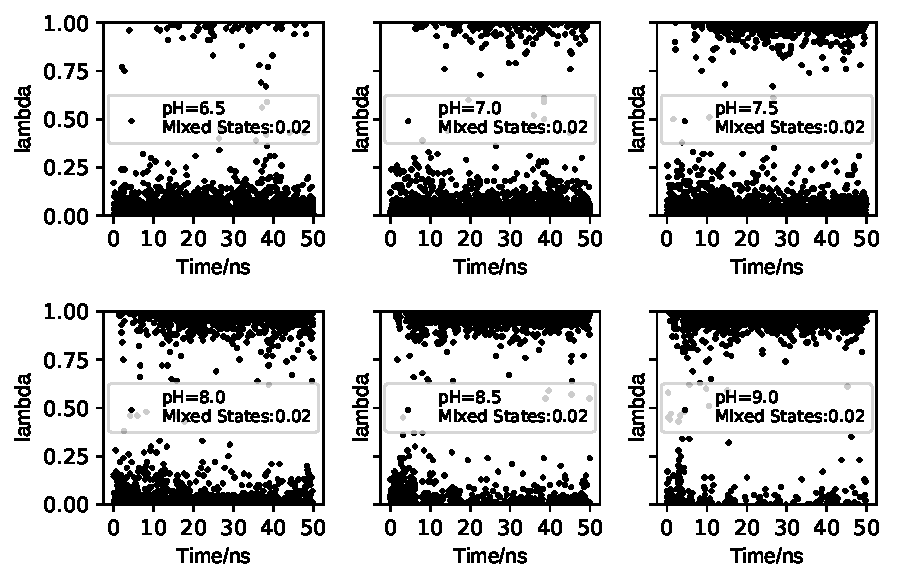
\includegraphics[width=3.6in]{figs/btk_c481_lambdavstime.pdf}
    \caption{\textbf{Time series of the $\lambda$ value for Cys481 in the BTK kinase.} 
    The data were saved every 20 ps (taken from Ref \cite{Liu_Shen_2021_J.Med.Chem.}). 
    The pH conditions and fractions of mixed states ($0.2 \le \lambda \le 0.8$) are given. 
    The plots show that the protonation-state sampling at all pH conditions 
    converge after $\sim$10 ns.
    }
\label{Fig:lambda_time}
\end{figure}
 %--------------------------------------------- 
 
To facilitate analysis of the lambda files, we developed a Python tool \href{https://gitlab.com/shenlab-amber-cphmd/cphmd-analysis}{cphmd\_anal.py}. 
This tool returns plots of the time series of unprotonated fractions and 
fitting of the unprotonated fractions to obtain {\pka's} (see discussion below).
For a trajectory at a specific pH, 
we can count the number of frames where a titratable residue $i$ is 
in the protonated or unprotonated state, which is defined 
as $\lambda_i < 0.2$ or $\lambda_i > 0.8$, respectively.
The unprotonated fraction of the residue ($S_i$)
is calculated as
\begin{equation}
S_i = \frac{N_i^{\rm Unprot}}{N_i^{\rm Prot} + N_i^{\rm Unprot}},
\end{equation}
where $N_i^{\rm Prot}$ and $N_i^{\rm Unprot}$ are
the number of protonated and unprotonated frames,
respectively.
Plotting the time series of the $S_i$ value informs
convergence of the protonation state sampling (Fig.~\ref{fig:intro}, step 5).
Once convergence is reached, the {\pka} of residue $i$
can be obtained by fitting the $S_i$ 
values at all simulation pH to 
the generalized Henderson-Hasselbalch equation,
\begin{equation}
S_i = \frac{1}{1+10^{n(\rm pK_{a,i} - pH)}},
\end{equation}
where $n$ is the Hill coefficient.
The resulting best fit is referred to as the titration curve (Fig.~\ref{fig:intro}, step 5).
A significant deviation of $n$ from 1 indicates cooperativity
($n>1$)
or anti-cooperativity ($n<1$) with a neighboring residue.
We note, in the past, $\lambda_i < 0.1$ and $\lambda_i > 0.9$ were used for
defining the protonated and unprotonated states \cite{Khandogin_Brooks_2005_Biophys.J.,Khandogin_Brooks_2006_Biochemistry}; 
however, our extensive studies (based on more than 100 proteins) showed 
that the calculated {\pka} value is not sensitive to the cutoff.

\subsection{Analysis of proton-coupled conformational dynamics and 
rationalization of the calculated {\pka} values}
A major application of 
CpHMD simulations is 
elucidation of pH-dependent or proton-coupled conformational dynamics, which 
in turn rationalizes the calculated {\pka} values. 
This practice can be best explained using an example. 
The pH replica-exchange GBNeck2-CpHMD simulations 
of the BTK kinase
\cite{Liu_Shen_2021_J.Med.Chem.}
gave a {\pka} of about 7.5 for Cys481,
which is one unit lower than the 
model {\pka} of cysteine -- the {\pka} value of an isolated cysteine 
fully exposed to solvent.
Analysis of the pH replicas (i.e., trajectories at different pH conditions) 
revealed that Cys481 accepts hydrogen bonds (h-bond) from 
Asn481 and Thr410 when it is in the deprotonated 
thiolate state (Fig.~\ref{Fig:analysis}a).
Note, these h-bonds are absent in the crystal structure (PDB 3pj3).
Following this observation, we plotted the deprotonated fractions 
of Cys481 at different pH conditions (Fig.~\ref{Fig:analysis}b)
and the occupancies of the h-bond formation 
between Cys481 and Asn484 or Thr410
(Fig.~\ref{Fig:analysis}c).
A comparison between the pH-dependent deprotonation
and h-bond formation demonstrates that the two are correlated, i.e., 
deprotonation of Cys481 is coupled to the h-bond formation.
It also suggests that the {\pka} downshift of Cys481 relative to the model value
can be attributed to the stabilization of the deprotonated thiolate state 
by the h-bond formation with Asn484 and Thr410.
We note, while implicit-solvent based CpHMD simulations have been 
successfully applied to {\pka} predictions and rationalization, 
hybrid-solvent and all-atom CpHMD simulations offer more accurate 
description of conformational dynamics.
We refer the user to the studies listed in Table~\ref{Table:applications} as examples.  


 %--------------------------------------------- 
\begin{figure}[htb!]
    \centering
    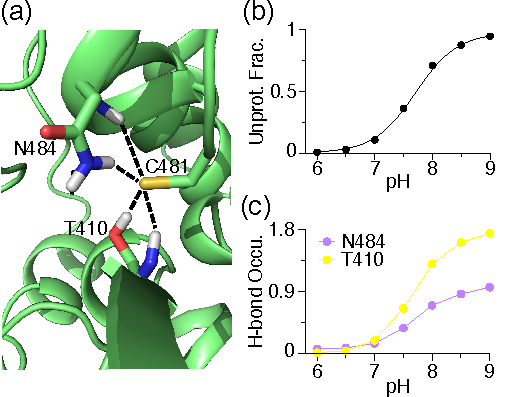
\includegraphics[width=3.3in]{figs/analysis_example.pdf}
    \caption{\textbf{An example analysis of proton titration of a cysteine and coupling with conformational dynamics.}
    (a) A zoomed-in view of the structural environment of Cys481 in the BTK kinase taken from the trajectory at pH 9. 
    The h-bonds with Asn484$\cdots$Cys481 and Thr410$\cdots$Cys481 are shown. 
    The pH 9 replica is used. 
    (b) The unprotonated fractions of Cys481 at different pH conditions. The titration curve represents the best fit to the Henderson-Hasselbalch equation. 
    (c) Occupancy of the h-bond formation between Cys481 thiolate and Asn484 or Thr410
    at different pH conditions. 
  Reprinted with permission from Liu, Zhan et al.\cite{Liu_Shen_2021_J.Med.Chem.} 
    Copyright {2021} American Chemical Society.
    }
\label{Fig:analysis}
\end{figure}
 %--------------------------------------------- 
 




\section{Parameterization of model titration} 
% - Jack/Ruibin
CpHMD is a relative free energy simulation approach, whereby the potential of mean force (PMF) of deprotonation of
a titratable amino acid in the protein environment is calculated relative to that of a reference, i.e., a model compound or peptide in solution
\cite{Lee_Brooks_2004_Proteins,Khandogin_Brooks_2005_Biophys.J.}. 
Model compounds, which were used in the early development of CpHMD methods
\cite{Lee_Brooks_2004_Proteins,Khandogin_Brooks_2005_Biophys.J.,Huang_Shen_2016_J.Chem.TheoryComput.},
are blocked single amino acid residues \ce{CH3CO}-X-\ce{NH2} or \ce{CH3CO}-X-\ce{CONH2},
where X represents a titratable amino acid.
In the development of the hybrid-solvent CpHMD \cite{Wallace_Shen_2011_J.Chem.TheoryComput.} and GBNeck2-CpHMD \cite{Huang_Shen_2018_J.Chem.Inf.Model.,Harris_Shen_2019_J.Chem.Inf.Model.}, 
model peptides 
\ce{CH3CO}-AAXAA-\ce{NH2} were used to take advantage of recent experimental data \cite{Thurlkill_Pace_2006_ProteinSci.,Platzer_McIntosh_2014_J.Biomol.NMR}.
Since in the CpHMD simulation, a model PMF is subtracted,
simulation of a model compound or peptide should return a zero PMF at the pH value equal to the model {\pka}.
In other words, protonated and deprotonated states are sampled with equal probabilities ($S\approx0.5$).
To ensure this is the case, the model PMF needs to be accurately determined.

To obtain the model PMF $U^{\rm mod}$, we use a free energy 
simulation method called thermodynamics integration,
in which the mean forces at different values of $\theta$ (for single site titration)
or $\theta$ and $x$ for double site titration
% $\langle\partial U/\partial\theta|_{\theta_i}\rangle$,
are calculated and then analytically
integrated to obtain $U^{\rm mod}$.
The single site titration model is applied
to Cys and Lys. The latter has equivalent protons, so one is selected for titration.
There are two types of double site titration model. His sidechains have two titratable nitrogens with different microscopic {\pka's}, while
carboxylate sidechains (Asp and Glu) have two titratable oxygens but identical microscopic {\pka's}.
These three titration models require
different forms of $U^{\rm mod}$ and methods of fitting.

\subsection{Protocol of parameterization for single site model titration}
For running TI simulations to obtain parameters, we set the options \textbf{prlam} to FALSE, \textbf{prderiv} to TRUE, and \textbf{phtest} to TRUE in the phmdin file, vph{\_}theta to 0 in the phmdstrt file.
For a single site titration model (e.g., Cys and Lys), 
we run CpHMD simulations at
$\theta_i=\left(0.4,0.6,0.785,1.0,1.2,1.4\right)$.
Each simulation is run for 10 ns, from which the mean forces
$\langle\partial U/\partial\theta|_{\theta_i}\rangle$
are calculated. 
Fitting of the mean forces  
to the following analytic form of $\partial U/\partial\theta$ (Eq.~\ref{Eq:dU_dtheta}) returns the two parameters $A$ and $B$ (Fig.~\ref{Fig:parm_cys}).

\begin{equation}
    \frac{\partial U}{\partial\theta}=2A\sin\left(2\theta\right)\left(\sin^{2}\theta-B\right).
    \label{Eq:dU_dtheta}
\end{equation}
As an example, Fig.~\ref{Fig:parm_cys} shows the fitting result for the GBNeck2-CpHMD titration of  Cys model peptide.
We note, fitting should be performed in the $\theta$ space (and not $\lambda$ space) to reduce errors.
 %--------------------------------------------- 
\begin{figure}[htb!]
    \centering
    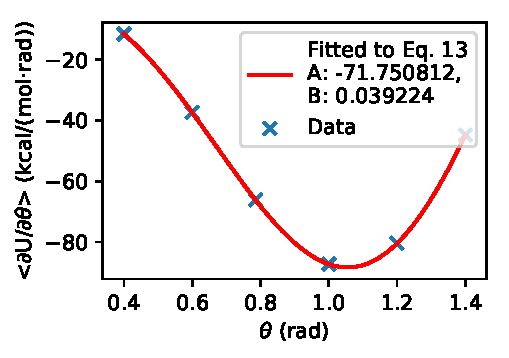
\includegraphics[width=3.3in]{figs/cys_parm.pdf}
    \caption{\textbf{Example of fitting A and B parameters for a single site titration model.}
    }
\label{Fig:parm_cys}
\end{figure}
 %--------------------------------------------- 

\paragraph{Protocol of parameterization for histidine model titration}
For a double site titration model 
with two different microscopic \pka's
(e.g. His), the two-dimensional PMF (Eq.~\ref{eq:double}) can be reduced to the
following form
\cite{Khandogin_Brooks_2005_Biophys.J.},

\begin{align}
U^{\rm mod}= & A_{10}\lambda^{2}x^{2}+2\left(A_{1}B_{1}-A_{0}B_{0}\right)\lambda x \nonumber \\ & + 2\left(A_{0}B_{0}-A_{1}B_{1}-A_{10}B_{10}\right)\lambda^{2}x \nonumber \\ & + A_{1}\lambda^{2}-2A_{1}B_{1}\lambda,
\label{eq:PMF_his}
\end{align}
where $\lambda=sin^2\theta$ and $x=sin^2\theta^x$. 
The six parameters $A_{0}$, $B_{0}$, $A_{1}$,  $B_{1}$, $A_{10}$, and $B_{10}$ are the parameters
in the quadratic functions
that describe the one-dimensional processes
\cite{Khandogin_Brooks_2005_Biophys.J.}.
$A_0$ and $B_0$ correspond to \ce{HIP <=> HID},
i.e., titration at N$\epsilon$;
$A_1$ and $B_1$ correspond to \ce{HIP <=> HIE},
i.e., titration at N$\delta$;
and $A_{10}$ and $B_{10}$ correspond to the tautomer interconversion \ce{HIE <=> HID}.


\textbf{Step 1.}
To obtain $A_0$ and $B_0$, we 
run TI simulations by fixing
$\theta^{x}$ at 0 ($\lambda=0$, HID, N$\delta$ is protonated), varying
$\theta$ at $\left(0.0,0.2,0.4,0.6,\\
0.785,1.0,1.2,1.4,1.5708\right)$, and fitting
the resulting mean forces to the following one-dimensional function,
\begin{equation}
    \frac{\partial U}{\partial\theta}=2A_{0}\sin\left(2\theta\right)\left(\sin^{2}\theta-B_{0}\right).
\end{equation}

\textbf{Step 2.}
To obtain $A_1$ and $B_1$,
we run TI simulations by fixing
$\theta^{x}$ at 1.5708 ($\lambda=1$, HIE, N$\delta$ is protonated), varying
$\theta$ at $\left(0.0,0.2,0.4,0.6,\\
0.785,1.0,1.2,1.4,1.5708\right)$, and 
fitting
 to the following one-dimensional function,
\begin{equation}
    \frac{\partial U}{\partial\theta}=2A_{1}\sin\left(2\theta\right)\left(\sin^{2}\theta-B_{1}\right).
\end{equation}

\textbf{Step 3.}
To obtain $A_{10}$ and $B_{10}$, we run TI simulations by fixing $\theta$ at 1.5708
($\lambda=0$, HIP, doubly protonated His),
varying $\theta_{x}$ at $\left(0.0,0.2,0.4,0.6,0.785,1.0,1.2,1.4,1.5708\right)$ 
and fitting the resulting mean forces
 to the following one-dimensional function,

\begin{equation}
    \frac{\partial U}{\partial\theta^{x}}=2A_{10}\sin\left(2\theta^{x}\right)\left(\sin^{2}\theta^{x}-B_{10}\right).
\end{equation}

\paragraph{Protocol of parameterization for carboxylic acid model titration}
For double site titration models with two identical microscopic \pka's (e.g., Asp and Glu), the two-dimensional PMF (Eq.~\ref{eq:double})
can be reduced to the following form \cite{Khandogin_Brooks_2005_Biophys.J.},
% Equation...
\begin{equation}
\begin{split}
U^{\rm mod}(\lambda_i,x_i) =
&(R_1 \lambda_i^2 + R_2 \lambda_i + R_3)(x_i + R_4)^2 + R_5 \lambda_i^2 + R_6 \lambda_i
\end{split}\label{eq:carboxyl}
\end{equation}

where $R_1$, ..., $R_6$ are parameters that can be determined via one-dimensional fitting.

%   Determine R1 R2 and R3 by fitting A(lambda) to R1 lambda^2 + R2 lambda + R3
%     R4 = 0.5
%     Determine R5 by fitting A(x) to C1 x^2 + C2 x + R5
%     Determine R6 by fitting B(x) to C1 x^2 + C2 x + R6

\textbf{Step 1.} To generate the data for fitting,
we run TI simulations at the combinations of $\theta$ value of 0.0, 0.4, 0.6, 0.785, 1.0, 1.2, or 1.4
and $\theta^{x}$ value of 0.0, 0.4, 0.6, 0.785, 1.0, 1.2, 1.4, or 1.5708.

\textbf{Step 2.}
We obtain $A$ and $B$ parameters 
at each value of $\theta$, 
$A(\theta)$ and $B(\theta)$,
by fitting
$\left<\partial U/\partial\theta_{x}\right>$
at different $\theta^x$ values to
the derivative of the quadratic function,
% can be obtained at each value of $\theta$ by fitting $<\partial U/\partial\theta_{x}>$ to
\begin{equation}
    \frac{\partial U}{\partial\theta^{x}}=2A(\theta)\sin\left(2\theta_{x}\right)\left(\sin^{2}\theta_{x}-B(\theta)\right),
\end{equation}
where $A(\theta)$ and $B(\theta)$ are the $\theta$-dependent parameters.

\textbf{Step 3.}
We obtain $A$ and $B$ parameters 
at each value of $\theta^x$, $A(\theta^x)$ and $B(\theta^x)$,
by fitting
$\left<\partial U/\partial\theta\right>$
at different $\theta$ values,
% compute $A\left(\theta_{x}\right)$ and $B\left(\theta_{x}\right)$ at each value of $\theta_{x}$ by fitting $\partial U/\partial\theta_{x}$ to

\begin{equation}
    \frac{\partial U}{\partial\theta}=2A(\theta^x)\sin\left(2\theta\right)\left(\sin^{2}\theta-B(\theta^x)\right),
\end{equation}
where $A(\theta^x)$ and $B(\theta^x)$ are the parameters.

\textbf{Step 4.}
We obtain $R_{1}$, $R_{2}$, and $R_{3}$ by fitting $A(\theta_i)$ to

\begin{equation}
    A\left(\theta\right) = R_{1}\sin^{4}\theta + R_{2}\sin^{2}\theta+R_{3},
\end{equation}

\textbf{Step 5.}
We set $R_{4}=0.5$, because the two titrating sites are identical. We then obtain $R_{5}$ by fitting $A(\theta^x)$ to

\begin{equation}
    A\left(\theta^{x}\right)=a_{0}\sin^{4}\theta^{x}+a_{1}\sin^{2}\theta^{x}+R_{5},
\end{equation}
and obtain $R_{6}$ by fitting $B(\theta^x)$ to

\begin{equation}
    B\left(\theta^{x}\right)=a_{0}\sin^{4}\theta^{x}+a_{1}\sin^{2}\theta^{x}+R_{6},
\end{equation}

\subsection{Scripts for TI simulations and parameterization}
To facilitate TI simulations and parameter fitting, we implemented a Shell script 
\href{https://gitlab.com/shenlab-amber-cphmd/cphmd-tutorial/-/blob/main/parameterization/scripts/heat_equil_prod_param.sh}{heat\_equil\_prod\_param.sh} and a Python program 
\href{
https://gitlab.com/shenlab-amber-cphmd/cphmd-tutorial/-/blob/main/parameterization/scripts/cphmd_parm_fit.py}{cphmd\_parm\_fit.py}.
% The above parameterization settings are included in the heat\_equil\_prod\_param.sh script and the fitting procedure is included in the cphmd\_parm\_fit.py script, both in the parameterization/scripts folder of the \href{https://gitlab.com/shenlab-amber-cphmd/cphmd-tutorial/-/tree/main/parameterization/scripts}{cphmd-tutorial} gitlab repository. 
Here we use Cys to illustrate the usage.
% A general instruction to use them (here we use Cys as an example) is firstly to run

\begin{lstlisting}
$ ./min.scr cys
$ ./heat_equil_prod_param.sh cys
\end{lstlisting}

After minimization, heating, equilibration, and production thermodynamic integration, 
we obtain $\partial U/\partial\theta$ values saved in files with the extension .lambda as in the folder \href{https://gitlab.com/shenlab-amber-cphmd/cphmd-tutorial/-/tree/main/parameterization/single}{single} (single site titration). 
We then call the Python script to fit the A and B parameters.
 
\begin{lstlisting}
$ python cphmd_parm_fit.py single
\end{lstlisting}

Four files are generated: du.data, du.fit, du.png, and cphmd.parm. du.data contains the mean force data, du.fit contains the detailed fitting results, du.png is the plot of the fitting (Fig.~\ref{Fig:parm_cys}) , and cphmd.parm contains the A and B parameters that can be directly copied and pasted into the standard CpHMD parameter file. 
The instructions for parameterization of different models are described in the folder \href{https://gitlab.com/shenlab-amber-cphmd/cphmd-tutorial/-/tree/main/parameterization}{parameterization} and the example results are included, as in the folders 
\href{https://gitlab.com/shenlab-amber-cphmd/cphmd-tutorial/-/tree/main/parameterization/single}{single},
\href{https://gitlab.com/shenlab-amber-cphmd/cphmd-tutorial/-/tree/main/parameterization/his}{his},
and 
\href{https://gitlab.com/shenlab-amber-cphmd/cphmd-tutorial/-/tree/main/parameterization/carboxyl}
{carboxyl}. 
% Here is a single-column checklist that consists of multiple sub-checklists
% \begin{Checklists}

% \begin{checklist}{A list}
% \textbf{Single-column checklists are also straightforward by removing the asterisk}
% \begin{itemize}
% \item First thing let's do an item which breaks across lines to see how that looks
% \item Also remember
% \item And finally
% \end{itemize}
% \end{checklist}

% \begin{checklist}{Another list}
% \textbf{This is some further description.}
% \begin{itemize}
% \item First thing
% \item Also remember
% \item And finally
% \end{itemize}
% \end{checklist}

% \end{Checklists}



\section{Author Contributions}
%%%%%%%%%%%%%%%%
% This section mustt describe the actual contributions of
% author. Since this is an electronic-only journal, there is
% no length limit when you describe the authors' contributions,
% so we recommend describing what they actually did rather than
% simply categorizing them in a small number of
% predefined roles as might be done in other journals.
%
% See the policies ``Policies on Authorship'' section of https://livecoms.github.io
% for more information on deciding on authorship and author order.
%%%%%%%%%%%%%%%%
Henderson, Liu, Harris, Huang, de Oliveira, and Shen
together wrote the manuscript.
We thank Zhi Yue and Paween Mahinthichaichan for contributing example scripts for the hybrid-solvent CpHMD simulations of transmembrane proteins.
We thank Jason A. Wallace for a bash script to calculate {\pka} values and track the convergence of unprotonated fractions using Grace.
% % We suggest you preserve this comment:
% For a more detailed description of author contributions,
% see the GitHub issue tracking and changelog at \githubrepository.

%\section{Other Contributions}
%%%%%%%%%%%%%%%
% You should include all people who have filed issues that were
% accepted into the paper, or that upon discussion altered what was in the paper.
% Multiple significant contributions might mean that the contributor
% should be moved to authorship at the discretion of the a
%
% See the policies ``Policies on Authorship'' section of https://livecoms.github.io for
% more information on deciding on authorship and author order.
%%%%%%%%%%%%%%%

% (Explain the contributions of any non-author contributors here)
% % We suggest you preserve this comment:
% For a more detailed description of contributions from the community and others, see the GitHub issue tracking and changelog at \githubrepository.

\section{Potentially Conflicting Interests}
%%%%%%%
%Declare any potentially competing interests, financial or otherwise
%%%%%%%
The CpHMD-related software may be of interest to ComputChem LLC, for which
J.S. is a founder and scientific advisor. 
J.S. also serves on the scientific advisory board of EoCys LLC.

\section{Funding Information}
%%%%%%%
% Authors should acknowledge funding sources here. Reference specific grants.
%%%%%%%
We acknowledge financial support from the National Institutes of Health (R01GM098818 and R01CA256557 to Shen and R44GM134756 to Harris) and National Science Foundation (CBET1932963 to Shen). 
We thank Zhi (Shane) Yue for contributing the input files for the membrane-enabled hybrid-solvent CpHMD simulations.
We thank Paween Mahinthichaichan for providing comments on the input files for the membrane-enabled hybrid-solvent CpHMD simulations.


\section*{Author Information}
\makeorcid

\bibliography{cphmd}

%%%%%%%%%%%%%%%%%%%%%%%%%%%%%%%%%%%%%%%%%%%%%%%%%%%%%%%%%%%%
%%% APPENDICES
%%%%%%%%%%%%%%%%%%%%%%%%%%%%%%%%%%%%%%%%%%%%%%%%%%%%%%%%%%%%

%\appendix


\end{document}
